\documentclass{pracamgr}  
\usepackage{lmodern} 
\usepackage[polish]{babel} 
\selectlanguage{polish} 
\usepackage{fontspec}
\usepackage{minted}
\usepackage{algorithm}
\usepackage{algpseudocode}
\usepackage{dsfont}
\usepackage{mathrsfs}
\usepackage{listings}
\usepackage{hyperref}
\usepackage{amsmath, amsthm, amssymb}
\usepackage[ansinew]{inputenc}
\usepackage{svg}
\usepackage{eucal}
\usepackage[mathcal]{eucal}
\usepackage[mathscr]{eucal}
\usepackage{csvsimple}
%===========================================================================
%                         Needed to use >{\bfseries}
%===========================================================================
\usepackage{array}

%===========================================================================
%                         Used for table border
%===========================================================================
\usepackage{booktabs}

\hypersetup{
    colorlinks,
    citecolor=black,
    filecolor=black,
    linkcolor=black,
    urlcolor=black
}
\usepackage{graphicx}  
\usepackage{makeidx}
\makeindex
\linespread{1.5} 
 

\makeatletter
\def\l@lstlisting#1#2{\@dottedtocline{1}{1.5em}{3em}{#1}{#2}}
\makeatother

\renewcommand{\listalgorithmname}{Spis algorytmów}
\makeatletter
\renewcommand{\ALG@name}{Algorytm}
\makeatother
\renewcommand{\thealgorithm}{\arabic{chapter}.\arabic{algorithm}} 

\definecolor{grey}{gray}{0.9}
\definecolor{bg}{HTML}{FAFAFA}
\definecolor{darkgray}{HTML}{D5D5D5} 

\renewcommand*{\listlistingname}{Lista kodów źródłowych}
\makeatletter
\raggedbottom
\renewenvironment{minted@colorbg}[1]{
\linespread{1.0} 
\setlength{\fboxsep}{\z@}
\def\minted@bgcol{#1}
\noindent
\begin{lrbox}{\minted@bgbox}
\begin{minipage}{\linewidth}}
{\end{minipage}
\end{lrbox}%
\colorbox{\minted@bgcol}{\usebox{\minted@bgbox}}}
\makeatother

% Dane magistranta:

\author{Konrad Lisiecki}
\nralbumu{48211}
\title{Wycena opcji przy pomocy modeli zmienności stochastycznej} 
\kierunek{Finanse i rachunkowość}
\instytut{Ekonometrii}
\opiekun{dra hab. Łukasza Delonga, prof. SGH} 
\date{Warszawa 2016}   
\newtheorem{defi}{Definicja}[section]
\newtheorem{prop}{Własność}
 

%===========================================================================
%                             Bibliogrphy
%=========================================================================== 
\usepackage[style=numeric,sorting=none,defernumbers=true, backend=bibtex]{biblatex}
\addbibresource{biblio.bib}
 
%===========================================================================
%                               Listings
%===========================================================================
\renewcommand\listoflistingscaption{Spis kodów źródłowych}
\renewcommand\listingscaption{Kod źródłowy}

\usepackage{chngcntr}% http://ctan.org/pkg/chngcntr
\counterwithin{listing}{chapter}

%===========================================================================
%                           Begin of document 
%===========================================================================
\begin{document}
\maketitle

%===========================================================================
%                               Introduction
%===========================================================================
\cleardoublepage
\phantomsection
\chapter*{Streszczenie} 
\addcontentsline{toc}{chapter}{Streszczenie} \markboth{Summary}{}


Tematem pracy magisterskiej jest wycena opcji przy pomocy modeli zmienności stochastycznej. 
W standardowych modelach służących do wyceny opcji przyjmuje się (jak np. w modelu 
Blacka-Scholesa), że zmienność jest stała, niezależna od czasu. 
Jak dalekie jest to założenie od rzeczywistości pokazał chociażby ostatni kryzys 
ekonomiczny, gdzie kursy instrumentów finansowych wahały się o wiele bardziej niż w czasach
koniunktury gospodarczej. Stąd też, w bardziej ogólnych modelach służących do wyceny opcji uzmiennia 
się parametr opisujący zmienność instrumentów finansowych i uzależnia się go od czasu. 

W drugim rozdziale zostanie opisany model Hestona i sposób w jaki można go zastosować do wyceny 
opcji. Zostaną przedstawione kroki jakie należy poczynić, aby wycenić opcję przy pomocy tego modelu.
Pokazane zostaną również możliwości dalszych uogólnień modelu Hestona. 
Polegają one głównie na próbie uzależnienia od czasu tych wartości parametrów, które w 
modelu Hestona są stałe w czasie.

Trzeci rozdział jest poświęcony kalibracji modelu, czyli znalezieniu 
optymalnych wartości nieznanych parametrów modelu. Optymalna wartość jest w tym przypadku zdefiniowana
jako taka, dla której wartość opcji, wyliczonej na podstawie modelu Hestona, jest najbliższa wartości 
obserwowanej na rynku.

W czwartym rozdziale zostanie przedstawiony algorytm symulacji Monte Carlo. 
Wprowadzone zostanie pojęcie dyskretyzacji procesu stochastycznego, które jest kluczowym elementem
jeśli chodzi o dokładność i szybkość działania symulacji. 


Ostatni rozdział to już próba empirycznego zbadania zachowania modelu Hestona. Zostanie w nim 
porównana wartość dwóch opcji testowych oraz opcji na indeks \textit{S\&P500} wyznaczonych w oparciu o  
różne schematy dyskretyzacji.



%===========================================================================
%                               Table of contents
%===========================================================================
\cleardoublepage
\phantomsection
\addcontentsline{toc}{chapter}{Spis treści}
\tableofcontents


%===========================================================================
%                               Wprowadzenie
%===========================================================================
\chapter{Wprowadzenie}
\label{chap:introduction}
\begin{quote}

  We developed what is known a stochastic volatility model. 
  This is a model where the volatility as well as the 
  underlying asset price moves around in an unpredictable way.

\raggedleft\slshape John Hull \index{Hull, John}
\end{quote}
Niniejsza praca jest poświęcona modelom zmienności stochastycznej używanych przy wycenie opcji. 
Nasuwa się jednak pytanie, czym dokładnie są te modele? 
Jaka jest ich istota? Jaka motywacja stoi za ich powstaniem?


Bardzo zwięzłej, a zarazem trafnej odpowiedzi na te pytania udziela John Hull, 
jeden z pionierów dzisiejszych finansów ilościowych. Stwierdza on, zgodnie z przytoczonym 
powyżej cytatem, że są to modele, gdzie nie tylko cena aktywa bazowego, ale również jego zmienność, 
poruszają się w sposób nieprzewidywalny, losowy. 

W niniejszej pracy przedstawiony zostanie model Hestona, w którym zmienność nie jest wartością stałą 
oraz sposób wyznaczenia wartości opcji przy pomocy tego modelu.
Część empiryczna pracy jest z kolei próbą sprawdzenia, jak model, oraz narzędzia do jego stosowania, 
sprawdzają się w praktyce.

W dalszej części tego rozdziału, zostanie przedstawiona motywacja do rozwoju takich modeli oraz w jaki 
sposób wpływają one na dokładność analizy finansowej i efektywność rynków finansowych. 


\section{Rys historyczny} % (fold)
\label{sec:rys_historyczny}

Do lat '90 XX wieku podstawowym modelem do wyceny opcji był model Blacka-Scholesa. Opublikowany w 
1973  \cite{BlackScholes} roku artykuł, którego autorami 
byli \textbf{Fischer Black}\index{Black, Fisher} oraz \textbf{Myron Scholes}\index{Scholes, Myron},
był przełomowy dla teorii wyceny opcji.
U jego podstaw leży bardzo istotne założenie mówiące o tym, że zmienność instrumentów finansowych 
jest stała w czasie. 
Niestety, założenie to jest niezgodne z tym co możemy obserwować na rynkach finansowych. 
Można to szczególnie mocno zauważyć w czasie cyklicznie powtarzających się kryzysów finansowych.

Obserwowalna duża zmienność w czasie parametru zmienności na rynkach finansowych stała się podstawową 
motywacją wprowadzenia modeli wyceny
opcji, dla których zmienność nie jest ustalonym parametrem, a zmienną zależną od pewnych innych 
czynników. Pionierem w tym obszarze okazał się \textbf{Steven Heston}\index{Heston, Steven}, który w 
1993 opublikował pracę gdzie wprowadza nowy model wyceny opcji, w którym nie tylko proces cen 
instrumentu bazowego, ale również proces zmienności jest stochastyczny (losowy) i zależny od 
czasu \cite{Heston}. Na jego cześć, model ten w literaturze znany jest pod nazwą modelu Hestona.
 

\section{Wycena opcji na potrzeby rynków finansowych} % (fold)

Instrumenty pochodne, a w szczególności opcje, są dzisiaj bardzo ważną klasą instrumentów finansowych 
i stanowią znaczną część wartości obrotu na światowych giełdach.

Światowy rynek derywatów, który dziś jest warty około 450 mld EUR  \cite{GlobalDerMarket}, jeszcze 
około 25 lat temu był bardzo mały. Powstaje więc pytanie co wpłynęło na rozwój tego typu transakcji 
na globalnym rynku? Z punktu widzenia rynku finansowego jest jedno wytłumaczenie tego zjawiska:
instrumenty pochodne, a szczególnie opcje, pozwalają na handel przyszłym ryzykiem związanym z ruchem 
cen instrumentów bazowych. W związku z tym można wyróżnić dwa podstawowe 
zastosowania opcji: 

\begin{enumerate}
  \item jako element zarządzania ryzykiem (\textit{ang. hedging}),
  \item jako inwestycja.
\end{enumerate}

Pierwsze zastosowanie odnosi się do wymiany lub ograniczenia ryzyka rynkowego. Przedsiębiorstwa i 
instytucje finansowe używają opcji do 
ochrony przed niechcianymi, gwałtownymi ruchami instrumentów bazowych takich jak surowce, stopy 
procentowe czy kursy akcji. Wpływa to na 
\textbf{wygładzenie przepływów pieniężnych} (\textit{ang. cash flows}) w obrębie przedsiębiorstwa, co 
ma znaczenie w kontekście stabilności działalności 
podmiotu gospodarczego. Dla przykładu, 92\% spośród 500 największych przedsiębiorstw świata ogranicza 
ryzyko przy pomocy derywatów  \cite{GlobalDerMarket}.


Transakcje na rynku instrumentów pochodnych są szczególnie ważne z punktu widzenia 
ograniczenia \textbf{ryzyka walutowego}. Na rysunku \ref{fig:currencyRisk} przedstawiono kurs dolara 
amerykańskiego w stosunku do rosyjskiego rubla na przestrzeni ostatnich 20 lat.
Można na nim odnotować gwałtowne wahania kursu, które dla wielu przedsiębiorstw, nie stosujących 
instrumentów pochodnych w celu ograniczenia ryzyka walutowego, może oznaczać bardzo szybkie 
bankructwo. 
\begin{figure}
  \centering  
  \includegraphics[width=0.80\textwidth]{../output/figures/currencyUSDRUB.pdf}
  \caption{Kurs walutowy rosyjskiego rubla w stosunku do dolara amerykańskiego.}\label{fig:currencyRisk}
\end{figure} 
 
Instrumenty pochodne mogą być również postrzegane przez uczestników rynku jako inwestycja. 
Różnią się one od inwestycji w instrumenty bazowe w tym sensie, że można w nie inwestować bez ich 
fizycznego zakupu.
Ponadto stwarzają one możliwość inwestycji w instrumenty, których po prostu nie można kupić 
bezpośrednio. Dobrym na to przykładem są derywaty pogodowe, które umożliwiają ubezpieczenie przed 
spadkiem temperatury poniżej określonego poziomu.
Pozwalają one również inwestorom na zajęcie pozycji w danym instrumencie finansowym nawet wtedy, gdy 
spodziewają się spadku ich wartości. W żargonie inwestycyjnym zajęcie takiej pozycji jest znane pod 
nazwą zajęcia \textbf{pozycji krótkiej} (\textit{ang. short position}).


\section{Wycena opcji na potrzeby rachunkowości}
\label{sec:aspekty_finansowe}

Jedną z nadrzędnych zasad rachunkowości jest \textbf{zasada prawdziwego i rzetelnego obrazu}. Oznacza 
ona, że rachunkowość musi pokazywać rzetelny, czyli prawdziwy i wiarygodny
obraz stanu majątkowego danej spółki. Zewidencjonowana cena instrumentów pochodnych, a w 
szczególności opcji, powinna więc odzwierciedlać ich \textbf{rzeczywistą 
(godziwą) wartość} (\textit{ang. fair value}) na moment bilansowy. W praktyce oznacza to, że 
zaawansowane modele wyceny opcji można zastosować w dwóch działach rachunkowości: rachunkowości 
sprawozdawczej oraz rachunkowości zarządczej.


\subsection{Rachunkowość sprawozdawcza} % (fold)
\label{sub:rachunkowosc_sprawozdawcza}
Pierwszym źródłem zastosowania zaawansowanych form wyceny opcji jest rachunkowość sprawozdawcza.
Opcje będące w posiadaniu przedsiębiorstwa, jako aktywa finansowe, są integralnym składnikiem każdego 
sprawozdania finansowego. Na koniec 
każdego roku sprawozdawczego istnieje potrzeba określenia ich wartości w celach sprawozdawczych.
\textbf{Międzynarodowy Standard Sprawozdawczości Finansowej MSSR 13} 
(\textit{ang. IFRS\index{IFRS}, International Financial Reporting Standard}) 
nie określa dokładnie w jaki sposób takie opcje mają być wycenione. 
Określa jednak, że jednostka powinna użyć takiej metody, która odzwierciedla
rzeczywistą  wartość instrumentu finansowego na dany moment. MSSR 13 wyróżnia podstawowe podejścia 
do ich wyceny \cite{IFRS2013}:
\begin{enumerate}
  \item podejście dochodowe\index{Podejście dochodowe} (\textit{ang. income approach}),
  \item podejście rynkowe\index{Podejście rynkowe} (\textit{ang. market approach}),
  \item podejście kosztowe\index{Podejście kosztowe} (\textit{ang. cost approach}).
\end{enumerate}
Pierwsze z nich, \textbf{podejście dochodowe}, określa wartość godziwą instrumentu finansowego na 
podstawie bieżących oczekiwań rynkowych co do wartości 
przyszłych przepływów pieniężnych i zdyskontowania ich na moment bieżący. Najbardziej powszechnymi 
modelami w tym podejściu są modele Blacka-Scholesa 
oraz model dwumianowy  \cite{IFRS2013}. W ostatnich latach jednak, w dobie postępu technologicznego, 
coraz istotniejszą rolę odgrywają bardziej zaawansowane metody probabilistyczne
(jak będące tematem tej pracy metody bazujące na modelowaniu zmienności przy pomocy stochastycznych 
równań różniczkowych) oraz symulacje Monte Carlo  \cite{FairValue2010}.  


\subsection{Rachunkowość zarządcza} % (fold)
\label{sub:RachunkowoscZarzadcza}
Kolejnym źródłem zastosowania bardziej zaawansowanych form wyceny instrumentów finansowych jest 
rachunkowość zarządcza. 
W przypadku wielu opcji niepłynnych, z wbudowaną możliwością wcześniejszego wykupu, standardy 
rachunkowości sprawozdawczej dopuszczają
\textbf{wycenę wg. zamortyzowanego kosztu nabycia} (\textit{ang. cost approach}). Organy zarządcze 
przedsiębiorstwa potrzebują jednak znać jak najbardziej dokładną sytuację księgowo-finansową 
przedsiębiorstwa, aby móc podejmować trafne decyzje bieżące i rozwojowe z punktu widzenia spółki. 
Wycena opcji przy pomocy metod użytych w tej pracy, może dać bardziej dokładną wycenę instrumentów 
finansowych, a co za tym idzie, lepszy obraz kondycji spółki dla osób zarządzających.  



\section{Model Blacka-Scholesa\index{Model Blacka-Scholesa}}

Poprzednie podrozdziały opisywały elementy rzeczywistości ekonomicznej na który istotny wpływ może 
mieć przyjęta metodologia wyceny opcji. W tym pokażemy najbardziej powszechny model do wyceny opcji, 
model Blacka-Scholesa. 
\subsection{Klasyczny model Blacka-Scholesa} % (fold)
\label{sub:classicBS}

Rozważmy następujący model przedstawiający ewolucję ceny aktywa
bazowego w czasie oraz obligacji, jako instrumentu finansowego pozbawionego ryzyka:
\begin{equation}
  \label{eq:asset}
  dS_t = \mu S_t dt + \sigma S_t d W_t 
\end{equation}

\begin{equation}
  \label{eq:nonRiskAsset}
  dB_t = r B_t dt, B_0 = 1, S_0 = 1
\end{equation}
gdzie:
\begin{enumerate}
  \item $S_t$ - cena aktywa bazowego
  \item $B_t$ - cena aktywa pozbawionego ryzyka
  \item $\mu$ - dryft ceny aktywa bazowego
  \item $\sigma$ - zmienność aktywa bazowego
  \item $W_t$ - proces Wienera
\end{enumerate}


Model ten znany jest pod nazwą \textbf{modelu Blacka-Scholesa} i jest fundamentalnym 
narzędziem do wyceny opcji. Równanie \ref{eq:nonRiskAsset}  jest istotną częścią modelu, ponieważ 
określa miarę w jakiej wyceniamy daną opcję. W zdecydowanej większości przypadków jest to miara 
neutralna względem ryzyka (miara martyngałowa\index{Miara martyngałowa}). 
Rozwiązując równanie (\ref{eq:asset}) można wyznaczyć:
\begin{equation}
\label{eq:closedFormBlackSmallt} 
  S_T = S_0 e^{(r - \frac{1}{2} \sigma^2)t+\sigma W_t}
\end{equation}
Po rozwiązaniu równania (\ref{eq:nonRiskAsset}) otrzymujemy natomiast:
\begin{equation}
B_t = e^{rt}
\end{equation}
co odpowiada procesowi kapitalizacji stopą równej stopie oprocentowania aktywa wolnego od ryzyka.

Zgodnie z teorią wyceny opcji, jej wypłata $v$ w mierze neutralnej względem ryzyka (na moment $t = 0$) 
jest równa:

\begin{equation}
\label{eq:discounting}
 \frac{\mathbf{E}[v(S_T)]}{e^{rT}}
\end{equation}
gdzie dynamikę cen aktywa bazowego opisuje następujący proces opisany w równaniu (\ref{eq:asset}),
którego dryft względem miary martyngałowej wynosi $\mu = r$.

Jak więc wynika z tego równania cenę opcji określamy jako zdyskontowaną na moment zerowy wartość
oczekiwaną z wypłat opcji w momencie jej wygaśnięcia. 

\subsection{Założenia modelu Blacka-Scholesa} % (fold)
\label{sub:zalozenia_modelu_blacka_scholesa}

Model Blacka-Scholesa należy do najbardziej popularnych, a zarazem najprostszych modeli do wyceny 
opcji. Podczas gdy jego prostota jest jedną z jego największych zalet, to posiada on wiele założeń,
które nie przystają do rzeczywistości rynkowej. Pierwsza grupa to założenia dotyczące aktywów:
\begin{enumerate}
\item cena aktywów bazowych ma rozkład log-normalny,
\item zmienność aktywów bazowych jest stała i znana z góry,
\item akcje nie wypłacają dywidend.
\end{enumerate}
Z kolei druga grupa założeń odnosi się do rynku na którym dane aktywa występują.
\begin{enumerate}
\item na rynku nie ma możliwości osiągnięcia ponadnormatywnego zysku bez ryzyka (brak możliwości arbitrażu),
\item nie ma kosztów transakcyjnych,
\item stopa procentowa na rynku jest stała i znana z góry.
\end{enumerate}

Wszystkie te założenia sprawiają, że model Blacka-Scholesa, mimo, że pozwala na wyznaczenie ceny
opcji w postaci analitycznej, może nieprecyzyjnie wycenić wartość takiej opcji.
  
\subsection{Zmienność implikowana} % (fold)
\label{sub:zmienno_implikowana} 
Kalibracja jest jednym z najważniejszych elementów procesu wyceny opcji.
W przypadku modelu Blacka-Scholesa jedynym nieobserwowalnym parametrem jest zmienność $\sigma$ (
współczynnik dyfuzji). Można go wyznaczyć na jeden z dwóch sposobów:
\begin{enumerate}
  \item zmienność historyczna,
  \item zmienność implikowana.
\end{enumerate}

Zmienność historyczna jest średnią (ważoną) zmienności zaobserwowanej na rynku w czasie 
poprzedzającym moment wyceny.

Szczególnie interesującym przypadkiem jest jednak zmienność implikowana, ponieważ 
wyraża ona \textit{"przewidywania rynku"} co do wartości zmienności danego aktywa bazowego. 
Można ją w prosty sposób obliczyć przy użyciu analitycznego \textbf{wzoru Blacka-Scholesa} na 
wycenę opcji, który da się przedstawić jako:

\begin{equation}
  \label{eq:impliedVol}
  C_{obs} = C(S_0, T, K, \sigma_{imp}, r)
\end{equation}
Jak widać, wiedząc jaka jest cena opcji na podstawie danych rynkowych, równanie (\ref{eq:impliedVol}) 
staje się równaniem z jedną niewiadomą, z którego możemy wyliczyć $\sigma_{imp}$.

W przypadku bardziej skomplikowanych modeli, nieznanych parametrów może być dużo więcej. Wtedy też 
stosuje się bardziej zaawansowane techniki kalibracyjne, co będzie tematyką 
rozdziału \ref{chap:chapterModelCalibration}.
  % \autoref - ok but it uses the english name of chapter

\subsection{Wycena opcji europejskiej} % (fold)
\label{sub:subsection_name}
 
Mając wartości wszystkich parametrów modelu Blacka-Scholesa jesteśmy w stanie przystąpić
do wyliczenia wartości opcji. Można wyznaczyć wartość opcji europejskiej dla 
strony kupującej (\textit{and. long call option}). Wypłata ta wynosi:

\begin{equation}
  v(S_T) = max(S_T-K, 0)
\end{equation}

W powyższym wzorze $K$, czyli cena wykupu opcji jest parametrem, stąd też, aby 
wyliczyć wartość opcji należy obliczyć wartość instrumentu bazowego w momencie wygaśnięcia opcji.

W tym celu należy rozwiązać stochastyczne równanie różniczkowe (\ref{eq:asset}). Jak pokazano
w sekcji \ref{sub:classicBS}, wartość ceny aktywa bazowego na moment wygaśnięcia opcji możemy wyznaczyć 
przy pomocy następującego wzoru:
\begin{equation}
\label{eq:closedFormBlack} 
  S_T = S_0 e^{(r - \frac{1}{2} \sigma^2)T+\sigma \sqrt{T} X}
\end{equation}
gdzie: $X \sim N(0,1)$.
Fragment wzoru postaci $\frac{1}{2} \sigma^2 T$ znany jest natomiast pod 
nazwą \textbf{poprawki Ito}\index{Poprawka Ito} (\textit{ang. Ito correction}).
Odpowiada on za przejście z modelu deterministycznego, opisywanego przez równania różniczkowe
zwyczajne, do modelu losowego, które opisują stochastyczne równania różniczkowe.

W końcu, aby uzyskać cenę opcji na dany moment, stosujemy wzór (\ref{eq:closedFormBlack}). Otrzymujemy
\begin{equation}
  C = \frac{\mathbf{E}[v(S_0 e^{(r - \frac{1}{2} \sigma^2)T+\sigma \sqrt{T} X})]}{e^{rT}}
\end{equation}
gdzie:
\begin{itemize}
  \item $X \sim N(0,1)$,
  \item $C$ oznacza wartość opcji na moment zerowy $t = 0$.
\end{itemize}




\section{Stosowane podejścia w procesie wyceny opcji} % (fold)
\label{sec:}

Istnieją dwa główne sposoby używane podczas wyceny opcji: skorzystanie ze wzorów analitycznych 
lub przeprowadzenie symulacji. O ile dla modelu Blacka-Scholesa rozwiązanie analityczne istnieje, 
to dla modeli o bardziej złożonych formułach, takich jak model Hestona, takich rozwiązań nie ma. 

Dlatego też o wiele bardziej uniwersalnym rozwiązaniem problemu wyceny opcji jest podejście symulacyjne.
Niezależnie od rodzaju opcji, czy też modelu opisującego dynamikę cen aktywa bazowego, można 
wyróżnić podobne etapy symulacji. Zaliczamy do nich:
\begin{enumerate}
  \item Kalibracja modelu,
  \item Generowanie zmiennych losowych o ustalonym rozkładzie,
  \item Wyznaczenie wartości zmiennych losowych opisujących realizacje procesu stochastycznego,
  \item Estymacja wartości oczekiwanej wypłaty.
\end{enumerate}

Kalibracja modelu jest tematem rozdziału \ref{chap:chapterModelCalibration}, natomiast pozostałe 
elementy będą przedstawione w rozdziale nr \ref{chap:monteCarlo}, poświęconym metodzie Monte Carlo.





%===========================================================================
%
%                               Model Hestona
%
%===========================================================================
\chapter{Model Hestona\index{Model Hestona}}
\label{chap:hestonModel}

Obecnie jednym z najpopularniejszych modeli do wyceny opcji jest przedstawiony 
w rozdziale \ref{chap:introduction} model Blacka-Scholsa. Ceniony jest 
on ze względu na prostotę oraz wygodę użycia, kosztem jednak wielu upraszczających założeń. 
Jedno z nich, założenie o stałości zmienności jest modyfikowane w modelu Hestona, który jest 
tematem tego rozdziału.


\section{Motywacja} 
Jak zostało powiedziane we wstępie do niniejszego rozdziału, podstawowym modelem do wyceny opcji jest 
model Blacka-Scholesa.
Możemy w nim wyprowadzić wzór na cenę opcji europejskiej w postaci analitycznej. 

Jednym z założeń modelu Blacka-Scholesa jest założenie o stałej zmienności instrumentu bazowego, 
które okazuje się być nieprawdziwe w rzeczywistym świecie. Świadczy o tym chociażby
wykres nr \ref{fig:vix}, na którym wyraźnie widać duże wahania zmienności ceny instrumentu bazowego.
Jednym z pomysłów na
obejście tego problemu jest uzmiennienie stałej wartości wariancji w tym modelu. Dopuszczamy w ten 
sposób, aby dla dowolnego czasu parametr ten przyjmował różną wartość. Można to zrobić np. poprzez 
nadanie cech losowych parametrowi zmienności. 
W takim przypadku nie tylko proces ceny akcji byłby procesem 
stochastycznym, ale także sama zmienność byłaby definiowana przy użyciu procesu stochastycznego. 
Tak powstała nowa klasa modeli wyceny opcji o nazwie \textbf{modele zmienności stochastycznej} 
(\textit{ang. stochastic volatility models}), której podstawowym 
przedstawicielem jest model Hestona.



\begin{figure}
  \centering  
  \includegraphics[width=0.80\textwidth]{../output/figures/volatilitySANDP.pdf}
  \caption{Zmieność w czasie indeksu S\&P500}\label{fig:vix}
\end{figure} 

\section{Model Hestona}
Jak wspomniano w poprzednim rozdziale, model Hestona eliminuje podstawową wadę modelu Blacka-Scholesa 
jakim jest założenie o stałej zmienności w czasie.
W tym celu zmienność uzależniono od dodatkowego procesu losowego. W 
przypadku modelu Hestona współczynnik zmienności może być opisany następującym równaniem:
\begin{equation}
\label{eq:cir}
dv_t  = \kappa (\theta  - v_t)dt + \varepsilon \sqrt{v_t} dW_t^v 
\end{equation}

Proces $v$ zdefiniowany przy pomocy (\ref{eq:cir}) posiada 
\textbf{\textit{własność powrotu do średniej długoterminowej}} (\textit{ang. mean-reversion}). 
Jeżeli byśmy założyli, że zmienność nie ma własności powrotu do średniej, obserwowalibyśmy 
znaczną część aktywów ze zmiennością bardzo gwałtownie rosnącą lub będącą blisko zera.
Z tego powodu, gdy założymy że proces spełnia \textbf{warunek Fellera\index{Warunek Fellera}}:
\begin{equation}
2 \kappa \theta > \varepsilon^2
\end{equation}
proces jest ściśle dodatni \cite{TheLittleHestonTrap}. Zmienność wtedy będzie zawsze wartością większą
od zera, co jest zgodne z jej definicją.

Mając równanie opisujące proces zmienności można już przedstawić model Hestona, który ma postać:

\begin{equation}
\label{eq:heston1}
dS(t)  = r S(t) dt + \sqrt{v(t)} S(t) dW^S(t)
\end{equation}
gdzie wariancja $v_t$ jest opisana przez następujące równanie: 

\begin{equation}
\label{eq:heston2}
dv(t)  = \kappa (\theta - v(t))dt + \varepsilon \sqrt{v(t)} dW^v(t) 
\end{equation}
Procesy $dW^v(t)$ oraz $dW^S(t)$ są standardowymi procesami 
Wienera\index{Proces Wienera} i są 
skorelowane:

\begin{equation}
Cov[dW^S(t), dW^v(t)] = \rho dt 
\end{equation}
gdzie:

\begin{enumerate}
\item $r$ oznacza dryft (\textit{ang. drift}) ceny aktywa bazowego 
\item $\theta$ oznacza długoterminową wartość oczekiwaną $v_t$
\item $\kappa$ jest współczynnikiem szybkości powrotu do średniej (\textit{ang. rate of mean-reversion})
\item $\varepsilon$ oznacza zmienność zmienności procesu $v_t$
\end{enumerate}

W przedstawionym modelu występuje równanie $Cov[dW^S(t), dW^v(t)] = \rho dt $. Mówi ono o tym, że 
dwa procesy błądzenia losowego są ze sobą skorelowane przy pomocy stałego 
współczynnika korelacji $\rho$.
To założenie jest zgodne z rzeczywistością. Często możemy na rynkach finansowych zaobserwować 
następującą sekwencję zdarzeń: gdy cena rośnie gwałtownie w górę, zwiększa się zmienność, 
natomiast w okresach spokoju zmienność jest na relatywnie niskim poziomie.

Niestety, w odróżnieniu od modelu Blacka-Scholsa, dla modelu Hestona nie istnieje pełne rozwiązanie 
analityczne (istnieje tylko częściowe rozwiązanie analityczne). Wobec tego, aby 
wyliczyć wartość opcji, należy się posłużyć metodami numerycznymi.

\section{Aplikacja lematu Ito dla modelu Hestona}

Pracując z szeregami czasowymi często łatwiej jest operować na 
logarytmach procesu bazowego, czyli $\ln S(t)$.
Podstawowym narzędziem używanym w wykonywaniu takich transformacji jest lemat Ito.

Procesy stochastyczne opisane równaniami (\ref{eq:heston1}) i (\ref{eq:heston2}) są tak 
zwanymi \textbf{procesami Ito}
(\textit{ang. Ito process}), które ogólnie dają się przedstawić w 
następującej formie:
\begin{equation}
  dx = a(x,t) dt + b(x,t) dz
\end{equation}
gdzie $z$ jest ruchem Browna. W równaniu wystpuje jeszcze parametr $a$, o którym 
można myśleć jako o współczynniku opisującym
wielkości wzrostu procesu oraz parametr $b$, definiujący jak duża jest losowość w danym 
modelu.

Dla procesów zdefiniowanych zgodnie z tym równaniem, możemy 
stosować \textbf{lemat Ito} (\textit{ang. Ito lemma}). Możemy na niego patrzeć 
jako stochastyczny odpowiednik reguły łańcuchowej (\textit{ang. chaining rule}) znanej z 
klasycznego rachunku różniczkowego. 
Po zastosowaniu lematu Ito dla $S(t)$ otrzymujemy układ równań z logarytmem aktywa bazowego $\ln S(t)$:
\begin{subequations}
\begin{align}
d \ln S(t) &= \left( r - \frac{1}{2} v(t) \right) dt 
              + \sqrt{v(t)} SdW^S(t) \label{eq:HestonlnS} \\
dv(t)      &= \kappa (\theta - v(t))dt + \varepsilon 
              \sqrt{v(t)} dW^v(t)  \label{eq:HestonlnY}
\end{align} 
\end{subequations}
Aplikując do równania (\ref{eq:HestonlnS}) \textbf{dekompozycję Cholesky'ego} można
otrzymać następującą zależność:
\begin{equation}
\label{eq:HestonCholesky}
  \ln S(t + \Delta) = \ln S(t) + \left( r - \frac{1}{2} v(t) \right) dt 
              + \rho \sqrt{v(t)} dW^v(t) + \sqrt{1 - \rho^2} \sqrt{v(t)} dW(t)
\end{equation}
Gdzie $W^v(t)$ jest procesem Wienera i jest niezależny od $W(t)$.
Drugie równanie (\ref{eq:HestonlnY}) można natomiast przedstawić jako:
\begin{equation}
  v(t + \Delta)      = v(t) + \int_t^{t+\Delta} \kappa 
                        (\theta - v(u))du + \varepsilon 
                        \int_t^{t+\Delta}  \sqrt{v(t)} dW^v(u) du 
\end{equation}
Co można przekształcić do następującej postaci:
\begin{equation}
  \int_t^{t+\Delta}  \sqrt{v(t)} dW^v(u) du  = \varepsilon^{-1} \left(v(t+\Delta) 
  - v(t) - \kappa \theta \Delta + \kappa \int_t^{t+\Delta}  v(u) du \right)
\end{equation}
Podstawiając to równanie do równania (\ref{eq:HestonlnS}) otrzymujemy:
\begin{equation}
\begin{aligned}
\label{eq:HestonLnSDiscretization}
\ln S(t + \Delta) = & \ln S(t) + r \Delta + \frac{\rho}{\varepsilon} 
(v(t + \Delta)  - v(t) - \kappa \theta \Delta) + \\
& \Big( \frac{\kappa \rho}{\varepsilon} - \frac{1}{2} \Big)
\int_t^{t+\Delta} v(u) du + \sqrt{1-\rho^2} \int_t^{t+\Delta} \sqrt{v(u)}dW(u)
\end{aligned}
\end{equation}

Powyższe równanie przedstawia dokładny wzór na wartość aktywa 
bazowego $\ln S(t + \Delta) $ mając daną wartość $\ln S(t)$.
Jedyną trudnością w wyznaczeniu wartości aktywa bazowego w momencie
$t + \Delta$ stanowią dwie całki, które muszą zostać wyznaczone przy 
pomocy metod numerycznych. 

\section{Wzór opisujący cenę opcji w modelu Hestona}

W modelu Hestona można wyznaczyć cenę dla europejskiej opcji \textit{call} na moment t, 
gdzie $t \in [0, T]$. Można ją zdefiniować, w sposób analogiczny do modelu Blacka-Scholesa, jako 
\cite{Heston}:

\begin{equation}
\label{eq:HestonCharacteristicFirst}
  C(S, v, t) = SP_1 -K e^{-r(T-t)} P_2
\end{equation}
gdzie:

\begin{equation}
\label{eq:HestonProb}
  P_j (x, v, T; ln[K]) = \frac{1}{2} + \frac{1}{\pi} \int_{0}^{\infty} Re \bigg[ \frac{e^{-i \cdot \phi ln[K]} f_j(x, v, T; \phi) }{i \phi} \bigg] d \phi 
\end{equation}

\begin{equation}
  x = ln(S_t)
\end{equation}
Funkcje charakterystyczne mają postać: 

\begin{equation}
\label{eq:HestonCharacteristic}
  \begin{aligned}
f_j(x, v, T; \phi) &= e^{C_j(T-t; \phi) + D_j(T-t; \phi)v + i \phi x} \\
C_j (\tau; \phi)     &= r \phi i \tau + \frac{a}{\sigma^2} \bigg\{ (b_j - \rho \sigma \phi i + d_j) \tau - 2 \cdot ln \bigg[ \frac{1 - g_j e^{d_j r}}{1-g_j} \bigg] \bigg\} \\
D_j (r; \phi)        &= \frac{b_j- \rho \sigma \phi i + d_j}{\sigma^2} \bigg[ \frac{1 - e^{d_j \tau}}{1 - g_j e^{d_j \tau}} \bigg]   \\
g_j                &= \frac{b_j - \rho \sigma \phi i + d_j}{b_j - \rho \sigma \phi i - d_j} \\
d_j                &= \sqrt{(\rho \sigma \phi i  - b_j)^2 - \sigma^2(2 u_j \phi  i  - \phi^2)}.
  \end{aligned}
\end{equation}
gdzie:
\begin{itemize}
  \item  $ u_1 = \frac{1}{2}$
  \item  $ u_2 = -\frac{1}{2}$
  \item  $ a = \kappa * \theta$
  \item  $ b_1 = \kappa + \lambda - \rho * \sigma$
  \item  $ b_2 = \kappa + \lambda$
\end{itemize}
dla: $j = 1,2$.

Przedstawione powyżej równania (\ref{eq:HestonProb}) oraz 
(\ref{eq:HestonCharacteristic}) będą użyte podczas kalibracji modelu. Należy jednak zaznaczyć, że 
w literaturze istnieją inne postacie analityczne ceny $C(S, v, t)$, które są bardziej wydajne 
obliczeniowo. 
Wiąże się to z faktem, że np. w wyrażeniu (\ref{eq:HestonProb}) występują dwie funkcje podcałkowe. 
Można pokazać, że równanie to da się przedstawić przy pomocy tylko jednej całki.

\subsection{Uproszczony wzór ceny opcji w modelu Hestona} % (fold)
\label{sec:numeryczne_wyznaczenie_warto_ci_funkcji_charakterystycznej}

Ważnym elementem podczas kalibracji modelu jest jak najszybsze wyznaczenie ceny opcji dla danego
zestawu parametrów. 
Jedną z metod używanych w tym celu jest całkowanie funkcji występującej we wzorze na funkcję
charakterystyczną (\textit{ang. Direct Integration}). Polega ona na wyznaczeniu całki przy pomocy
numerycznej kwadratury, jak np. kwadratury Gaussa\index{Kwadratura Gaussa}. Można także zastosować
inną postać funkcji charakterystycznej, wyznaczoną przez Attariego \cite{Attari}\index{Attari,
Mukarram}, która jest bardziej efektywną metodą do jej obliczenia:
\begin{equation}
\label{eq:AttariCharacteristicFirst}
\begin{aligned}
  C(S_0, T, K) = S_0 &- \frac{1}{2} e^{-rT}K  \\ 
  &- e^{-rT} K 
  \left( \frac{1}{\pi} \int_0^{+\infty} Z d\omega \right)
    \end{aligned}
\end{equation}
gdzie:

\begin{equation}
\label{eq:AttariCharacteristic}
  Z = \frac{
(Re(\phi (\omega) )
+\frac{Im(\phi (\omega)}{\omega}
cos(\omega l (K)) +
(Im(\phi (\omega) - \frac{Re(\phi (\omega)}{\omega}
sin(\omega l (K))
}{1 + \omega^2}
\end{equation}
Jedynym ograniczeniem powyższego układu jest fakt, że równania 
(\ref{eq:HestonCharacteristicFirst}) - (\ref{eq:HestonCharacteristic}) pozwalają wyznaczyć wartość opcji w 
dowolnym momencie jej trwania. Równania 
(\ref{eq:AttariCharacteristicFirst}) - (\ref{eq:AttariCharacteristic}) z kolei nie mają tej własności, 
pozwalają wycenić opcję jedynie na moment zerowy.





\subsection{Mała pułapka Hestona} % (fold)
\label{sub:mala_pulapka_hestona}
W pewnych przypadkach podany wzór na wycenę opcji może charakteryzować się dużą niestabilnością
numeryczną. Główną przyczyną niestabilności jest istnienie wielu załamań i 
nieciągłości całkowanej funkcji. Zjawisko to zostało zauważone po raz pierwszy
przez Albrechera i znane jest w literaturze pod nazwą \textbf{małej pułapki Hestona} (\textit{ang. 
The little Heston trap}) \cite{albrecher2006little}.

\begin{figure}
\centering
  \includegraphics[width=0.80\textwidth]{../output/figures/AlbrecherHeston.png}
  \caption{Porównanie wyglądu fragmentu funkcji $P_j$ dla oryginalnej 
           postaci modelu Hestona i Albrechera. Źródło: \cite{rouah2013heston}.}
  \label{fig:AlbrecherHeston}
\end{figure}
W przypadku modelu Hestona funkcją, która zawiera wyrażenie podcałkowe, jest $P_j$. 
Wyrażenie to ma postać:

\begin{equation}
\label{eq:HestonProb}
  F_j(\phi) = Re \bigg[ \frac{e^{-i \cdot \phi ln[K]} f_j(x, v, T; \phi) }{i \phi} \bigg], 
\end{equation}
gdzie: $\phi > 0$.

Powyższy fragment dla pewnych danych może charakteryzować się dużą nieregularnością. 
Dla przykładu, na rysunku \ref{fig:AlbrecherHeston} przedstawiono wykres 
funkcji $P_j$ ilustrujący to zjawisko. Zestaw parametrów, dla których funkcja $P_j$
zachowuje się w ten sposób, jest następujący \cite{rouah2013heston}:
\begin{itemize}
  \item $\kappa = 1.5768$,
  \item $\sigma = 0.5751$,
  \item $\rho = −0.5711$,
  \item $\theta = 0.0398$,
  \item $v_0 =0.0175$.
\end{itemize}

Jak widać, funkcja zapisana w oryginalnej postaci 
modelu Hestona charakteryzuje się nieciągłością dla punktu $\phi \approx 3,6$. 
Natomiast funkcja zdefiniowana w alternatywnej postaci jest funkcją ciągłą i nie wykazuje
bardzo dużych załamań swoich wartości.


Aby otrzymać postać zaproponowaną przez Albrechera należy zastąpić 
niektóre części oryginalnego wzoru ekwiwalentnymi wyrażeniami.
Zmiana ta powoduje, że funkcja jest bardziej gładka i nie charakteryzuje się tak dużymi
załamaniami.

Pierwszym wyrażeniem wymagającym poprawy jest $D_j$ w równaniu (\ref{eq:HestonCharacteristic}). 
Zastępujemy je przez:


\begin{equation}
\label{eq:HestonLittleTrapD}
  \begin{aligned}
D_j (r; \phi)  &= \frac{b_j- \rho \sigma \phi i - d_j}
                  {\sigma^2} \bigg[ \frac{1 - e^{-d_j \tau}}{1 - c_j e^{-d_j \tau}} \bigg],  
  \end{aligned}
\end{equation} 
gdzie:

\begin{equation}
\label{eq:HestonLittleTrapCj}
  \begin{aligned}
c_j  &= \frac{1}{g_j} = \frac{b_j - \rho \sigma \phi i - d_j}{b_j - \rho \sigma \phi i + d_j}. \\
  \end{aligned}
\end{equation}
Wyrażenie $C_j$ należy natomiast zamienić następującym równaniem:

\begin{equation}
\label{eq:HestonLittleTrapC}
  \begin{aligned}
C_j (\tau; \phi)     &= r \phi i \tau + \frac{a}{\sigma^2} 
                    \bigg\{ (b_j - \rho \sigma \phi i - d_j) \tau - 
                    2 \cdot ln \bigg[ \frac{1 - c_j e^{-d_j r}}{1-c_j} \bigg] \bigg\}.
  \end{aligned}
\end{equation}
Wyrażenie $c_j$ w powyższym wzorze jest zdefiniowane 
w ten sam sposób jak w równaniu (\ref{eq:HestonLittleTrapCj}).

% subsection mała_pułapka_hestona (end)

\section{Współczynniki greckie\index{Współczynniki greckie}}

Z punktu widzenia uczestnika rynku finansowego, cena jest jedną z dwóch najważniejszych 
właściwości opcji. Drugą bardzo istotną kwestią jest sprawdzenie wrażliwości opcji na jednostkowe 
zmiany poszczególnych parametrów opcji.
Definiuje się więc pięć podstawowych współczynników, znanych w literaturze pod 
nazwą \textbf{współczynników greckich}.
Zaliczamy do nich \cite{Hull}:
\begin{enumerate}
  \item $\Delta$ (delta)
  \item $\Gamma$ (gamma)
  \item $\Theta$ (theta)
  \item $v$ (vega)
  \item $\rho$ (rho)
\end{enumerate}
 

Pierwszy ze współczynników, \textbf{Delta} $\Delta$, odpowiada na pytanie w jaki 
sposób zmieni się cena opcji w odpowiedzi na
jednostkową zmianę instrumentu bazowego:
\begin{equation}
  \Delta = \frac{\delta V}{\delta S}
\end{equation} 
Kolejny, \textbf{Gamma} $\Gamma$, definiuje wrażliwość delty na 
jednostkową zmianę ceny instrumentu bazowego:
\begin{equation}
  \Gamma = \frac{\delta \Delta}{\delta S} = \frac{\delta^2 V}{\delta^2 S}
\end{equation}
\textbf{Theta} $\Theta$, trzeci ze współczynników określa tak 
zwaną \textbf{wartość czasową opcji} (ang. option time value).
Opisuje go poniższy wzór:
\begin{equation}
  \Theta = \frac{\delta V}{\delta \tau}
\end{equation}
Przedostatni współczynnik grecki nosi nazwę \textbf{Vega} $v$ i określa wrażliwość wartości 
opcji na jednostkową zmianę poziomu
zmienności:
\begin{equation}
  v = \frac{\delta V}{\delta v}
\end{equation}
Ostatni wskaźnik \textbf{Rho} $\rho$ wskazuje na wrażliwość ceny na wahania stopy procentowej:
\begin{equation}
  \rho = \frac{\delta V}{\delta r}
\end{equation}
Należy zauważyć, że wzory analityczne wyznaczające wartość współczynników greckich nie zawsze istnieją. 
Okazuje się, że albo funkcja wypłaty opcji jest zbyt skomplikowana, albo sam model jest zbyt 
skomplikowany. Często też obydwa warunki występują jednocześnie. 

Współczynniki greckie są bardzo ważnymi narzędziami 
do zabezpieczenia (\textit{ang. hedging}\index{Hedging}) ryzyka 
związanego z inwestycją w instrumenty pochodne.
Do wyznaczenia wartości tych współczynników używa się metod Monte Carlo. Wynika to z faktu, 
że niemożliwe jest uzyskanie dla nich wzoru analitycznego, 
zwłaszcza dla bardziej skomplikowanych modeli jak model Hestona.

\section{Rozszerzenia modelu Hestona}

Model Hestona uogólnia założenie o stałości zmienności w czasie. 
Jednak pozostałe parametry wciąż pozostają na niezmienionym poziomie
co daje możliwość uzależnienia w czasie kolejnych stałych w modelu.
Ponadto, również wariancję w modelu Hestona można uzależnić nie tylko 
od jednego, ale od wielu procesów zmienności (\textit{ang. Multifactor Heston Models}).

Kolejną możliwością uogólnienia modelu Hestona to wprowadzenie do modeli zmienności stochastycznej
\textbf{skoków} (\textit{ang. stochastic volatility models with jumps})
Tego typu modele tworzą odrębną klasę modeli, a procesem, który najczęściej modeluje właściwość
skoków w tego typu modelach jest proces Poissona.

Celem tego rozdziału jest tylko zasygnalizowanie możliwych rozszerzeń modelu Hestona.
Mogą być one jednak zaimplementowane przy pomocy zaprojektowanego w tej pracy modułu 
do wyliczenia ceny opcji w oparciu o model Hestona. 

\subsection{Dwuczynnikowy model Hestona} % (fold)
\label{sec:modelDwuczynnikowy}
Model dwuczynnikowy Hestona został w 2009 zaproponowany prze
Petera Christoffersena \index{Christoffersen, Peter} \cite{Christoffersen}.
Opisuje go następujący układ równań:

\begin{equation}
dS_t  = r S_t dt + \sqrt{V_1} S dW_1 + \sqrt{V_2} S dW_2
\end{equation} 

\begin{equation}
dV_1  = (a_1 - b_1 V_1)dt + \sigma_1 \sqrt{V_1} dW_3 
\end{equation}

\begin{equation}
dV_2  = (a_2 - b_2 V_2)dt + \sigma_2 \sqrt{V_2} dW_4 
\end{equation}

W modelu tym zmienna $W_1$ jest skorelowana z $W_3$ na poziomie korelacji $\rho_1$, natomiast
zmienna $W_2$ z $W_4$ jest skorelowana na poziomie $\rho_2$. Ponadto, $W_1$ oraz $W_2$ są ze sobą 
nieskorelowane. Z tego względu (właściwość
liniowości wariancji dla zmiennych losowych o kowariancji równej $0$) wariancja stopy zwrotu z aktywa
bazowego jest sumą wariancji:

\begin{equation}
  Var_t[dS/S] = (V_1 + V_2)dt = Vdt
\end{equation}

Jak wynika z powyższych wzorów cena akcji instrumentu bazowego zależy teraz nie od jednego, a od 
dwóch procesów zmienności.
Jednym z powodów dla którego chcielibyśmy wprowadzać dodatkowe zmienne jest fakt, że model
Hestona nie zawsze jest w stanie dostosować się do `uśmiechu zmienności'  implikowanej, w 
szczególności dla krótkich okresów  \cite{HestonExtensions}.


\subsection{Modele zmienności stochastycznej ze skokami} % (fold)
\label{sec:modele_zmienno_ci_stochastycznej_ze_skokami}
 
Kolejnym modelem, który rozszerza model Hestona jest model zmienności stochastycznej ze skokami.

Jest wiele powodów wprowadzenia skoków do równania modelującego cenę aktywa bazowego, a wśród nich 
możemy wymienić `grube ogony' rozkładu stóp zwrotu. Zgodnie z danymi empirycznymi ogony rozkładu stóp 
zwrotu aktywa bazowego są grubsze od tych występujących w rozkładzie normalnym.

Kolejną przyczyną wprowadzenia skoków do modelu Hestona jest kształt płaszczyzny zmienności implikowanej
(\textit{ang. volatility surface}) dla opcji o krótkim terminie do wykupu. W rzeczywistości ma ona 
bardziej skośny kształt niż to wynika z danych wygenerowanych przez model Hestona. 
Bates \cite{Bates} rozszerzył więc model Hestona o dodatkowy element, który ma niwelować opisaną wadę.

Model ten różni się od modelu Hestona tylko składnikiem definiującym skoki, jednak dla
porządku podajemy jego pełną definicję:
\begin{equation}
dS_t  = \mu S_t dt + \sqrt{v_t} S_t dW^S_t + S_{t-} Y_t dN_t^S.
\end{equation}
Wariancję $v_t$ opisuje równanie: 

\begin{equation}
dv_t  = \kappa (\theta - v_t)dt + \varepsilon \sqrt{v_t} dW_t^v.
\end{equation}
Procesy $dW_t^v$ oraz $dW_s^v$ są skorelowane na poziomie $\rho$:

\begin{equation}
Cov[dW^S_t, dW^v_t] = \rho dt.
\end{equation}
W powyższych wzorach $N_t^S$ jest procesem Poissona, $Y_t$ oznacza wysokość skoku, 
natomiast $S_{t-}$ oznacza, że skok dotyczy wartości procesu ceny przed skokiem.

Motywacją stojącą za wprowadzeniem skoków do modelu jest chęć uchwycenia momentów o 
szczególnej i gwałtownej zmianie ceny instrumentu bazowego. Dla indeksu S\&P500, omawianego w tej pracy,
skoki są szczególnie widoczne podczas kryzysów ekonomicznych. 



 


%===========================================================================
%                       Kalibracja modelu Hestona
%===========================================================================
\chapter{Kalibracja modelu}
\label{chap:chapterModelCalibration}



Przed przystąpieniem do wyznaczenia ceny opcji w modelu Hestona potrzebujemy uzyskać zestaw 
parametrów ceny akcji i zmienności. Problem wyznaczenia parametrów modelu 
nazywamy \textbf{problemem kalibracji} modelu.  

Jak widzieliśmy w rozdziale \ref{chap:introduction}, zadanie kalibracji dla modelu Blacka-Scholesa 
nie jest zadaniem skomplikowanym. Do oszacowania mamy tylko jeden parametr, który należy wyznaczyć na 
podstawie danych giełdowych i odwróconego wzoru na cenę opcji w modelu Blacka-Scholesa.

Dla modelu Hestona sytuacja wygląda nieco bardziej skomplikowanie. Zamiast jednego mamy do 
oszacowania pięć parametrów:
$V(0),\kappa, \theta, \sigma, \rho$.  

Jednym ze sposobów kalibracji modelu jest technika symulowanego 
wyżarzania (ang. simulated annealing)\index{Symulowane wyżarzanie}. Należy ona do 
grona stochastycznych metaheurystyk, \index{Metaheurystyka} które pomagają w rozwiązaniu problemów 
optymalizacyjnych (a takim właśnie problemem 
jest kalibracja modelu, gdzie chcemy zminimalizować wartość funkcji będącej różnicą wartości funkcji 
wynikającej z modelu i z rynku). Kolejnym sposobem kalibracji jest powszechnie stosowana nielinowa
metoda najmniejszych kwadratów. 
Właśnie ta metoda zostanie użyta w niniejszej pracy w celu wyznaczenia parametrów modelu.

Warunkiem efektywnego zastosowania powyższej metody jest znalezienie szybkiego obliczeniowo sposobu 
wyznaczania wartości opcji w 
modelu Hestona. Ponieważ podejście symulacyjne jest zbyt czasochłonne w procesie kalibracji, stosuje 
się równanie opisujące cenę opcji w formie jawnej. Równanie to opisano w rozdziale \ref{chap:hestonModel}.


\section{Deterministyczne sposoby kalibracji modelu} 
Pierwsza grupa algorytmów używanych w celu skalibrowania modelu Hestona należy do grupy metod 
deterministycznych.
Algorytmy te polegają na tym, że mając zadany punkt startowy wyszukiwany jest najbardziej optymalny
punkt w sposób nielosowy.
Najważniejszym przedstawicielem tej klasy jest Nieliniowa Metoda Najmniejszych Kwadratów 
(\textit{ang. Nonlinear Least Squares}).


\subsection{Nieliniowa Metoda Najmniejszych Kwadratów \index{Nieliniowa Metoda Najmniejszych Kwadratów}}

Optymalizacja zadanej funkcji celu polega na dopasowaniu danych empirycznych do zadanej funkcji celu 
według pewnego zadanego kryterium (zadanej miary). 
Jedną z najczęściej używanych miar jest ta polegająca na minimalizacji kwadratów błędów estymacji. 
Najprostszą metodą z tej klasy jest (liniowa) Metoda Najmniejszych Kwadratów (MNK). \index{Metoda 
Najmniejszych Kwadratów} W świecie rzeczywistym jednak ciężko sobie wyobrazić, aby tego typu 
specyfikacja problemu modelowała wszystkie możliwe relacje ekonomiczne. 

Ważnym ograniczeniem tej metody jest założenie o liniowej zależności pomiędzy zmiennymi. 
Gdy jednak zrezygnujemy z tego założenia, w wyniku otrzymamy 
nową metodę zwaną \textbf{Nieliniową Metodą Najmniejszych Kwadratów}.
Dla porządku, poniżej podajemy jej formalną specyfikację \cite{NLS}.

\begin{defi}
 Rozważmy pewną nieliniową funkcję $f: R^l \times \Theta \rightarrow R$, gdzie $\Theta$ oznacza 
 przestrzeń parametrów i jest podprzestrzenią $R^k$. Wtedy $y$ można przedstawić jako:
\begin{equation}
  y = f(x; \beta) + e(\beta)
\end{equation}
gdzie funkcja $e(\beta)$ oznacza \textbf{błąd specyfikacji}. 
Mając $N$ obserwacji $y$ oraz wektor $x$, zdefiniujmy wektory \textbf{$y$} 
oraz $\mathbf{f(x_1, ... x_N; \beta)} $
w następujący sposób:

\begin{align}
\mathbf{y} &=  \begin{bmatrix}
         y_1 \\
         y_2 \\
         \vdots \\
         y_N
        \end{bmatrix},
&
\mathbf{f(x_1, x_2, \ldots, x_N; \beta}) &=  \begin{bmatrix}
         f(\mathbf{x_1; \beta})\\
         f(\mathbf{x_2; \beta})\\
         \vdots \\
         f(\mathbf{x_N; \beta})
        \end{bmatrix}
\end{align}
Wobec tego, 

\begin{equation}
 \mathbf{y = f(x; \beta) + e(\beta)}
\end{equation}
gdzie $\mathbf{e(\beta)}$ oznacza teraz wektor błędów specyfikacji.



\end{defi}


\subsection{Estymator NMNK}
Mając podaną specyfikację NMNK, chcielibyśmy znaleźć jego estymator, czyli taką statystykę, która 
najlepiej dopasowuje dane $(y_t, \mathbf{x_t}}), t = 1, ..., T$ względem zadanego kryterium. Tak jak 
w przypadku klasycznej MNK, także dla NMNK  
zminimalizujemy wartość sumy kwadratów różnic między wartościami empirycznymi, a teoretycznymi:
\begin{equation}
Q_T(\mathbf{\beta}) = \frac{1}{T} \sum_{t=1}^T [y_t - f(\mathbf{x_t, \beta})]^2
\end{equation}
Aby znaleźć ekstremum danej funkcji, należy znaleźć wektor parametrów spełniający 
następujące warunki:
\begin{itemize}
  \item Warunek pierwszego rzędu:
\begin{equation}
  \nabla Q_T(\mathbf{\bar{\beta}}) = 0
\end{equation}
  \item Warunek drugiego rzędu:
\begin{equation}
  \nabla^2 Q_T(\mathbf{\bar{\beta}}) > 0 
\end{equation}
\end{itemize}

Metoda minimalizująca wartość $Q_T(\mathbf{\beta})$ jest znana 
jako \textbf{estymator NMNK} (\textit{ang. NLS estimator}) i oznaczamy ją przez $\hat{\beta}_T$.

Należy zauważyć, że w przypadku metody MNK, jej estymator można podać w postaci wzoru
analitycznego. Nie zawsze jest to jednak możliwe dla metody NMNK, co wynika wprost z nieliniowości 
jej specyfikacji: pochodnych funkcji nieliniowych (potrzebnych do wyznaczenia warunku pierwszego rzędu) 
nie zawsze da się wyznaczyć analitycznie.


\begin{figure}
  \centering
  \includegraphics[width=0.80\textwidth]{../output/figures/NLS.pdf}
  \caption{Przykład dopasowania funkcji wykładniczej do danych}
  \label{fig:volatilitySurface}
\end{figure}




\subsection{Kalibracja modelu Hestona przy pomocy NMNK}

Warunek pierwszego rzędu dla funkcji nieliniowych z reguły
jest trudny do wyznaczenia analitycznego. Stosuje się więc metody numeryczne, które są metodami 
iteracyjnymi i zaczynającymi przeszukiwać przestrzeń w zadanym punkcie startowym (wybór punktu 
startowego może mieć duże znaczenie dla zbieżności metody).

Jedną z najprostszych jest \textbf{metoda największego spadku} 
(\textit{ang. steepest descent algorithm}). Jej idea polega na tym, że w 
każdym kroku algorytm stara się podążać w kierunku największego spadku, aż 
napotka ekstremum lokalne. Definicję pojedynczego kroku w tej metodzie 
przedstawia poniższe równanie:


\begin{equation}
  x_{k+1} = x_k - \alpha_k \nabla f(x_k)
\end{equation}
gdzie: $\nabla f(x_k)$ oznacza gradient, czyli pole wektorowe pokazujące kierunki najszybszego 
wzrostu.


Inna popularną metodą gradientową jest metoda Gaussa-Newtona. Różni się ona od metody największego 
spadku nieco innym schematem wyboru kierunku spadku. Nie używa ona gradientu, 
lecz informacji o krzywiźnie funkcji w danym punkcie (poprzez obliczenie pochodnych).
Podobnie jak dla metody najszybszego spadku definiujemy krok algorytmu jako:


\begin{equation}
  x_{k+1} = x_k - (J_k^TJ_k)^{-1}J_k e_k
\end{equation}
gdzie: $J_k$ oznacza macierz Jakobiego, czyli macierz pochodnych cząstkowych, 
natomiast $e_k$ jest wektorem wartości rezydualnych.

Obie te metody są wydajnymi sposobami obliczania ekstremów lokalnych, jednak mają swoje wady.
Zgodnie z literaturą \cite{LM}, pierwsza metoda dobrze się zachowuje dla punktów początkowych 
znajdujących się daleko od ekstremum, natomiast druga metoda zachowuje się dobrze w punktach 
położonych blisko ekstremum. 

Z połączenia dwóch przedstawionych powyżej metod powstał tzw. \textbf{algorytm Levenberga–Marquardta} 
(\textit{ang. Levenberg–Marquardt algorithm}). Został on zaimplementowany w pakiecie \textit{Matlab} 
jako funkcja \textit{lsqnonlin} \cite{NonLinear}\index{lsqnonlin}. Funkcja ta jest użyta w procesie 
kalibracji, którego wynik jest przedstawiony w rozdziale nr \ref{r:sp}, a jej nagłówek 
jest widoczny poniżej:

\begin{listing}[H]
\inputminted[mathescape, linenos, numbersep=5pt, bgcolor=bg, frame=lines, framesep=2mm]{matlab}
{listings/lsqnonlin.m}
\caption{Nagłówek funkcji \textit{lsqnonlin}}
\label{lst:lsqnonlin}
\end{listing}

Algorytm Levenberga–Marquardta można przedstawić jako niewielką modyfikację metody Gaussa-Newtona:


\begin{equation} 
  x_{k+1} = x_k - (J_k^TJ_k + \lambda I)^{-1}J_k e_k
\end{equation}
gdzie: $\lambda$ jest nazywany 
\textbf{współczynnikiem kombinacji} (\textit{ang. combination coefficient}) i 
ma zawsze wartość dodatnią.

Gdy współczynnik $\lambda$ jest bliski zero, to metoda ta zbiega do metody Gaussa-Newtona. 
Z kolei dla dużej wartości współczynnika $\lambda$ metoda zbliża się do metody największego spadku
z wartością współczynnika $\alpha_k$:

\begin{equation}
  \alpha_k = \frac{1}{\lambda}
\end{equation}
Tak jak pozostałe algorytmy z rodziny metod gradientowych, metoda Levenberga–Marquardta zachowuje się
bardzo dobrze dla funkcji z jednym ekstremum. Gdy jednak funkcja ma wiele ekstremów, bardzo ważną
rolę odgrywa punkt początkowy. Maksimum globalne możemy znaleźć tylko w przypadku jego bliskiego
położenia.



\subsection{Parametry wejściowe do procesu kalibracji}

Aby wyznaczyć parametry modelu jako dane wejściowe podajemy następujące dane dostępne na rynku:
\begin{enumerate}
  \item cenę wykonania opcji (ang. strike),
  \item czas wygaśnięcia opcji (ang. maturity).
\end{enumerate}
Są to dane wejściowe jakie należy podać w formie wektorów o jednakowej długości.
Ponadto, do metody kalibrującej parametry modelu Hestona należy podać następujące 
wartości skalarne:
\begin{enumerate}
  \item wartość aktywa bazowego w momencie $t=0$,
  \item stopę wolną od ryzyka.
\end{enumerate}

\section{Techniki przyspieszenia procesu kalibracji} %
Kalibracja modeli zmienności stochastycznej jest zadaniem czasochłonnym obliczeniowo. 
Istnieją jednak sposoby na jego przyspieszenie. W podrozdziale zostaną przedstawione 
dwie główne techniki stosowane w tym celu: uproszczenie równania opisującego cenę opcji 
w modelu oraz spamiętywanie powtarzających się wartości funkcji charakterystycznej.


\subsection{Zastosowanie uproszczonej formy ceny opcji w modelu Hestona} % (fold)
\label{sec:uproszczona_forma}

Pierwszą techniką przyspieszającą proces kalibracji jest zastosowanie uproszczonej formy ceny opcji w 
modelu Hestona. 
Opisana w podrozdziale \ref{sec:numeryczne_wyznaczenie_warto_ci_funkcji_charakterystycznej} 
formuła ma dwie przewagi nad tą przedstawioną przez Hestona:
\begin{enumerate}
  \item Formuła zawiera tylko jedną funkcję podcałkową do obliczenia
  \item Funkcja podcałkowa ma wyrażenie kwadratowe w mianowniku, co daje szybszą zbieżność  \cite{Attari}
\end{enumerate}

\subsection{Spamiętywanie wartości funkcji charakterystycznej}
Postać funkcji charakterystycznej dla modelu Hestona jest bardzo czasochłonna obliczeniowo. 
Zawiera ona wiele skomplikowanych funkcji z punktu widzenia procesora:
\begin{itemize}
  \item dwie zespolone funkcje eksponencjalne
  \item dwie zespolone funkcje logarytmiczne
  \item zespoloną funkcję pierwiastkową
\end{itemize}
Nie są one zależne w żaden sposób od parametrów wejściowych procedury kalibrującej (ceny wykupu oraz 
czasu do wygaśnięcia), dlatego też nie ma powodu ich wyliczania dla każdej pary. 
Stosuję się więc ich spamiętywanie (\textit{ang. caching}).
Tak wyglądałby schemat działania metody kalibrującej \cite{AcceleratingHeston} przed zastosowaniem 
techniki spamiętywania:
\begin{algorithm}[H]
\caption{Schemat metody kalibrującej}\label{euclid}
\begin{algorithmic}[1]
  \State Iteruj po wszystkich wartościach czasu do wygaśnięcia opcji
  \State Iteruj po wszystkich wartościach ceny wykonania opcji
  \State Iteruj po wszystkich wartościach $\omega_i, i = 1, ..., U $ użytych do numerycznego wyznaczenia całki z równania   
  \State Oblicz wartość funkcji charakterystycznej w punkcie $\omega_i$
  \State Oblicz wartość całki w punkcie $\omega_i$
  \State Oblicz wartość opcji
\end{algorithmic}
\label{alg:simulatedAnnealing}
\end{algorithm}
Zauważmy, że wartość funkcji charakterystycznej w punkcie $\omega_i$ jest niezależna od czasu do 
wygaśnięcia opcji oraz ceny jej wykonania. Można zatem zoptymalizować krok w linii nr 4. Tak wygląda 
algorytm po zastosowaniu spamiętywania wartości funkcji charakterystycznej:

\begin{algorithm}[H]
\caption{Schemat metody kalibrującej ze spamiętywaniem}\label{euclid}

\begin{algorithmic}[1]
  
  \State Iteruj po wszystkich wartościach czasu do wygaśnięcia opcji
  \State Iteruj po wszystkich wartościach ceny wykonania opcji
  \State Iteruj po wszystkich wartościach $\omega_i, i = 1, ..., U $ użytych do numerycznego wyznaczenia całki z równania   
  \State Jeżeli jesteśmy w pierwszym kroku pętli, oblicz i zapamiętaj $\omega_i$
  \State Jeżeli nie jesteśmy w pierwszym kroku pętli, odczytaj zapisaną wartość $\omega_i$
  \State Oblicz wartość całki w punkcie $\omega_i$
  \State Oblicz wartość opcji

\end{algorithmic}
\label{alg:simulatedAnnealing}
\end{algorithm}




Na podstawie powyżej przedstawionych pseudokodów widać, że obliczamy funkcję 
charakterystyczną tylko raz, podczas pierwszego obrotu wewnętrznej pętli.



\section{Stochastyczne sposoby kalibracji modelu}
Przedstawione jak do tej pory algorytmy optymalizacyjne są algorytmami deterministycznymi.
Często jednak wprowadzenie czynnika losowego może poprawić ich efektywność lub dokładność. Jednym z
nich jest algorytm symulowanego wyżarzania, który nadaje się szczególnie dobrze do efektywnego
przeglądu tych klas funkcji, które mają nieregularną powierzchnię, tzn. takich, w których występuje
wiele ekstremów lokalnych.

\subsection{Symulowane wyżarzanie}

Jak opisano we wstępie, większość algorytmów, nigdy nie osiągną ekstremum
globalnego. Jedną z takich technik jest \textit{hill climbing}\index{Hill climbing}, która jednak 
osiąga dobre rezultaty tylko dla funkcji o wypukłej powierzchni. W tym algorytmie możemy poruszać się
tylko w kierunku maksimum lokalnego, co skutecznie uniemożliwia przeszukiwanie przestrzeni o wielu
ekstremach.

Wprowadza się zatem odstępstwo od tej reguły. Pod pewnym warunkiem można przeskoczyć od 
jednego wzgórza do drugiego, co pomaga algorytmowi poruszać się w obrębie wielu ekstremów lokalnych.
Można to osiągnąć poprzez wprowadzenie losowości do algorytmu. 

Otrzymujemy w ten sposób stochastyczne metody optymalizacji, a jednym z najważniejszych 
reprezentantów tej klasy metod jest przedstawiony w 1983 roku przez Kirkpatricka 
\cite{Kirkpatrick},  algorytm symulowanego wyżarzania  (\textit{ang. simulated annealing}). 
Motywacją dla jego powstania jest szeroko stosowany w metalurgii \textbf{proces chłodzenia}
\index{Proces chłodzenia} ciała stałego (\textit{ang. cooling process}). Składa on się z
następujących etapów  \cite{ChenBin}:

\begin{enumerate}
  \item Podnoszenia temperatury, tak, że substancja stała się topi,
  \item Powolnego wychładzania substancji tak, że poruszające się tam cząsteczki gromadzą się w stanie o najmniejszej energii.
\end{enumerate}

Dobrym przykładem obrazującym działanie algorytmu jest wyobrażenie skaczącej piłki na terenie 
o nierównej powierzchni.
W warunkach niskiej siły grawitacji, piłka odbijając się od powierzchni leci wysoko w górę i może
przeskoczyć z jednej doliny do drugiej, natomiast odwrotnie się dzieje w przypadku wysokiej siły
grawitacji. Wtedy piłce trudniej jest się oderwać od powierzchni i wydostać się z doliny. Podobnie
sprawa ma się w przypadku cząsteczek umieszczonych w metalu: przy wysokiej 
temperaturze mogą się one swobodnie przemieszczać w ciele, natomiast wraz ze spadającą temperaturą 
stają się one uwięzione w jednym punkcie.

Przedstawiona idea rozwiązuje szereg problemów podczas rozwiązywania problemów optymalizacyjnych, a 
najważniejszym z nich jest potencjalne istnienie wielu ekstremów lokalnych.

\begin{algorithm}[H]
\caption{Algorytm symulowanego wyżarzania}\label{euclid}

\begin{algorithmic}[1]
  
  \State Zainicjuj temperaturę początkową $T_0$;
  \State Zainicjuj rozwiązanie początkowe $x_0$;
  \State Dla każdego poziomu temperatury $T_K$:
  \State \hspace{\algorithmicindent} Zdefiniuj funkcję $\pi_k(x) = e^{- \frac{G(x)}{T_k}}$
  \State \hspace{\algorithmicindent} Wykonaj $n$ iteracji:
  \State \hspace{\algorithmicindent} \hspace{\algorithmicindent} Zaakceptuj nowe rozwiązanie 
          $x_{k+1}$ z pr-stwem $min(1, \frac{\pi_k{x_{k+1}}}\pi_k{{x_{k}}}$);
  \State  Jeżeli $T_{k+1} < T_{min}$:
  \State  \hspace{\algorithmicindent} Zakończ algorytm;
  \State  W przeciwnym przypadku:
  \State  \hspace{\algorithmicindent}  Skocz do linii 3 z temperaturą $T_{k+1}$ oraz rozwiązaniem $x_{k+1}$;

\end{algorithmic}
\label{alg:simulatedAnnealing}
\end{algorithm}

Działanie algorytmu symulowanego wyżarzania można zobaczyć na schemacie nr 
\ref{alg:simulatedAnnealing}. Poniżej pokrótce omówimy działanie algorytmu.
Funkcja ma dwa argumenty: pierwszy argument dotyczy wysokości temperatury początkowej (i ewentualnie
szybkości chłodzenia systemu), natomiast drugi rozwiązanie początkowe.
Najważniejszą częścią algorytmu jest pętla 4-6. 
Centralną rolę odgrywa tam reguła Metropolisa, która mówi czy bieżące rozwiązanie powinno być 
zaakceptowane czy nie (najważniejszym parametrem jest bieżąca temperatura systemu). 
Linie 7-10 to już tylko sprawdzenie warunku końcowego: jeżeli temperatura jest dostatecznie 
niska to kończymy algorytm, ponieważ wiemy, że i tak nie znajdziemy bardziej optymalnego rozwiązania.



%===========================================================================
%                       Metody Monte Carlo
%===========================================================================
\chapter{Metody Monte Carlo}
\label{chap:monteCarlo}

Przeprowadzenie wyceny opcji w modelu Hestona jest zadaniem znacznie trudniejszym
niż w przypadku modelu BS. Wynika to z tego, że w modelu Hestona trajektoria 
ceny instrumentu bazowego jest zależna od trajektorii jego zmienności. To pociąga za sobą
konsekwencje w procesie wyceny opcji, ponieważ teraz należy najpierw wygenerować trajektorię
zmienności, a dopiero później, na tej podstawie, generować trajektorię cen instrumentu bazowego.

Aby jednak wygenerować trajektorię cen, musimy umieć przedstawić równanie opisujące
zmienność aktywa bazowego w postaci \textit{zdyskretyzowanej}.

W tym rozdziale pokażemy jak efektywnie, przy pomocy schematów dyskretyzacji i symulacji Monte Carlo, 
wyznaczyć najpierw trajektorie procesu zmienności i aktywa bazowego, a następnie wyliczyć wartość
opcji o zadanym schemacie wypłaty.

\section{Prosta metoda Monte Carlo (MC)}
\label{sec:mc}

Rozdział zaczynamy od przedstawienia prostej metody 
Monte Carlo (\textit{ang. Crude Monte Carlo (CMC)}) \cite{Niemiro}.

\begin{defi}
Załóżmy, że mamy wygenerowane $n$ zmiennych losowych $X_1, ..., X_n$ o takim samym rozkładzie. 
Wtedy estymatorem wartości oczekiwanej $EX$ jest średnia z próby:
\begin{equation}
  \hat{\theta}_n = \sum_{i=1}^n \frac{X_i}{n}
\end{equation}
Inaczej mówiąc, aproksymujemy prawdziwą wartość oczekiwaną 
\textbf{średnią z próby} (\textit{ang. sample mean}).
\end{defi}


Zgodnie z Mocnym Prawem Wielkich Liczb mamy pewność, że estymator 
$\hat{\theta}_n \rightarrow EX$ prawie na pewno, wtedy gdy $n \rightarrow \infty$. 
Oznacza to, że estymator $\hat{\theta}_n $ jest \textbf{mocno zgodnym} 
estymatorem $EX$ \cite{Glasserman}.



\section{Generowanie zmiennych losowych}
\label{sec:genRV}

Efektywność przedstawionej metody Monte Carlo wynika z łatwości uzyskania dowolnie dużej
ilości liczb losowych. 
W tym podrozdziale zostaną pokazane najważniejsze sposoby generowania liczb losowych.


\subsection{Generowanie zmiennych losowych o rozkładzie normalnym}

Pierwszym krokiem jaki należy podjąć podczas przeprowadzania symulacji Monte Carlo jest 
wygenerowanie zmiennych losowych o ustalonym rozkładzie.

W przypadku wyceny opcji w modelu Blacka-Scholesa potrzebna jest umiejętność generowania liczb 
(pseudo)losowych z rozkładu normalnego. Znamy wiele algorytmów generowania liczb o rozkładzie
normalnym, wśród których można wyróżnić:
\begin{enumerate}
  \item metoda odwrotnej dystrybuanty,
  \item metoda Boxa-Mullera,
  \item metoda biegunów (\textit{ang. Marsaglia\index{Marsaglia, George} Polar Method}) \cite{Marsaglia},
  \item algorytm ziggurat.
\end{enumerate}

Mimo, że najbardziej wydajną metodą generowania liczb pseudolosowych o rozkładzie normalnym jest 
algorytm ziggurat, a najbardziej ogólną jest metoda odwrotnej dystrybuanty (pozwala na generowanie 
liczb o dowolnym rozkładzie pod warunkiem umiejętności wyznaczenia funkcji odwrotnej do dystrybuanty 
danego rozkładu), w tym rozdziale zostanie przedstawiona metoda biegunów.

Jest ona wariantem metody Boxa-Mullera\index{Box, George}\index{Muller, Edgar}. W przeciwieństwie do 
metody Boxa-Mullera nie zawiera ona funkcji $sin$ oraz $cos$, dlatego też jest znacznie wydajniejsza 
obliczeniowo \cite{Korn}.
Polega ona na wybraniu losowego punktu $(x,y)$ z rozkładu jednostajnego spełniającego warunek:
\begin{equation}
  \{(x, y): s = x^2 + y^2 < 1\}
\end{equation}
Wtedy liczby losowe o standardowym rozkładzie normalnym otrzymujemy stosując następujące 
przekształcenia:
\begin{equation}
  u_1 = x \sqrt{\frac{-2 \ln(s)}{s}}, u_2 = y \sqrt{\frac{-2 \ln(s)}{s}}
\end{equation}
Pseudokod \ref{lst:polarMethodLst} przedstawia zarys algorytmu generowania zmiennej losowej o standardowym rozkładzie
normalnym przy pomocy wyżej opisanego schematu \cite{joshi2008c++}. 

\begin{algorithm}[H]
\caption{Generowanie zmiennej losowej o standardowym rozkładzie normalnym zgodnie z metodą biegunów}
\label{lst:polarMethodLst}

\begin{algorithmic}[1]

  \State do \{
  \State \hspace{\algorithmicindent} $x = 2.0$ $\cdot$ Uniform(0,1)
  \State \hspace{\algorithmicindent} $y = 2.0$ $\cdot$ Uniform(0,1)
  \State \hspace{\algorithmicindent} $s = x^2 + y^2$
  \State \}
  \State while ($s \geq 1.0$)
  \State return $x \cdot \sqrt{\frac{-2 \ln(s)}{s}}$

\end{algorithmic}
\label{alg:polarMethod}
\end{algorithm}





\subsection{Generowanie skorelowanych ruchów Browna}
\label{sec:genRB}

Ważną kwestią, która pojawia się podczas implementacji modelu Hestona, jest generowanie skorelowanych 
ruchów Browna.

Dla przypadku dwuwymiarowego problem redukuje się do 
następującej postaci:

\begin{equation}
  \varepsilon_1 = x_1
\end{equation}
\begin{equation}
  \varepsilon_2 = \rho x_1 + x_2 \sqrt{1-\rho^2}
\end{equation}
gdzie:
\begin{enumerate}
  \item $x_i$ - wygenerowana zmienna losowa z rozkładu normalnego
  \item $\rho$  - współczynnik korelacji
\end{enumerate}




\section{Schematy dyskretyzacji}


Model Hestona, opisany w Rozdziale \ref{chap:hestonModel}, opisuje dynamikę procesów cen aktywa 
bazowego oraz jego zmienności w postaci ciągłej.
Chcąc jednak wycenić opcję \textit{call} przy pomocy metody Monte Carlo, należy wygenerować 
trajektorie procesów w nim występujących w postaci dyskretnej. 

Następujący podrozdział będzie poświęcony metodom dyskretyzacji występującym w literaturze.

\subsection{Generowanie trajektorii procesu stochastycznego}
Generowanie trajektorii procesów stochastycznych występujących w modelu Hestona polega na
wygenerowaniu pary wektorów losowych o elementach $(S(t), v(t))$, dla każdego $t \in \mathscr{T}$, 
gdzie $\mathscr{T}$ jest danym zbiorem dyskretnych punktów w czasie 
$\mathscr{T}  = \{t_i\}^N_{t=1}$. Aby wygenerować taką parę wektorów losowych wystarczy znać 
odpowiedź na inne fundamentalne pytanie: jak można wygenerować punkty wektorów losowych 
$(S(t+ \Delta), v(t+ \Delta))$
mając dany punkt $(S(t), v(t))$? Mając taki schemat, można go iteracyjnie lub rekurencyjnie aplikować 
dla każdego kolejnego punktu począwszy od zadanego elementu $(S(0), v(0))$, 
aż do otrzymania punktu $(S(T), v(T))$.
Kolejne podrozdziały będą odpowiedzią na pytanie jakie schematy można zastosować w celu 
efektywnego przejścia od $(S(t), v(t))$ do $(S(t+ \Delta), v(t+ \Delta))$.

Używamy w nich notacji $\hat{S}, \hat{v}$ dla oznaczenia dyskretnych trajektorii procesów 
stochastycznych $S, v$.

\subsection{Dyskretyzacja Eulera}

Poniższe równanie nr \ref{h:euler} przedstawia \textbf{dyskretyzację Eulera} równania 
zmienności \cite{Broadie}:
 
\begin{equation}\label{h:euler}
v_{i+1}  = v_i + \kappa (\theta - v_i) \Delta t + \varepsilon  \sqrt{v_i} \Delta W^{v}_{i+1}.
\end{equation}
gdzie: $\Delta W^{v}_{i+1} = W^{v} (t_i+\Delta) - W^{v} (t_i)$.

Powyższe równanie jest wynikiem dyskretyzacji procesu ciągłego do procesu dyskretnego. Przejście
takie jest jednak podatne na numeryczne błędy zaokrągleń. Niestety, pomimo faktu, że 
proces zmienności $v_t$ w postaci ciągłej nie może osiągnąć wartości ujemnej, po 
dyskretyzacji okazuje się, że wartość ta może być ujemna. 

Aby tego uniknąć, wszędzie tam, gdzie możliwe jest wystąpienie ujemnej 
wartości zmienności $v_i$, zastępujemy ją poprzez $v_i^+ = \max(v_i, 0)$. Operacja taka nazywana jest 
\textbf{pełnym obcięciem} (\textit{ang. full truncation})\index{Full truncation} \cite{Lord}.
Rozwiązanie to, jak do tej pory, okazało się być najbardziej dokładnym i 
efektywnym w swojej klasie \cite{Malham}. Ostatecznie więc, wzór opisujący dynamikę $v_i$ przyjmuje 
postać:

\begin{equation}\label{h:eulerNonZero}
v_{i+1}  = v_i + \kappa (\theta - v_i^+) \Delta t + \varepsilon \sqrt{v_i^+} \Delta W^{v}_{i+1}.
\end{equation}

Mając wygenerowaną trajektorię zmienności, można przystąpić do zdyskretyzowania równania opisującego 
dynamikę cen aktywa bazowego, jednakże pamiętając o tym, aby zmienność zawsze była wartością 
dodatnią. 
Mając to na uwadze, równanie (\ref{h:eulerAssetPath}) opisuję dynamikę cen instrumentu bazowego w 
postaci dyskretnej:

\begin{equation}\label{h:eulerAssetPath}
S_{i+1} = S_i + S_i r \Delta t + S_i \sqrt{v_i^+}  \Delta W_{i+1}^S.
\end{equation}
gdzie: $\Delta W^{S}_{i+1} = W^{S} (t_i+\Delta) - W^{S} (t_i)$.
  
Aby wygenerować przyrosty procesu Wienera wykorzystujemy fakt, że $W_{i+1}  - W_{i}$ są niezależne 
względem pozostałych przyrostów. 
Każdy taki przyrost ma rozkład normalny o średniej równej $0$ oraz odchyleniu standardowym 
równym $\sqrt{\Delta t}$. 
Dlatego do wygenerowania przyrostów procesu Wienera można zastosować metody przedstawione w 
podrozdziale \ref{sec:genRV} \cite{Glasserman}.


\subsection{Schemat Andersena - dyskretyzacja procesu zmienności}
\label{sec:algorytm_andersena}
O ile schemat dyskretyzacji Eulera jest najprostszym do implementacji schematem dyskretyzacji, to ma 
on wiele wad jak np.  
Algorytm Andersena \cite{Andersen}, zwany również pod nazwą schematu 
kwadratowo-wykładniczego (\textit{ang. Quadratic Expotential (QE) scheme}),
znacząco niweluje te wady, czyniąc proces dyskretyzacji bardziej dokładnym przy niewiele wolniejszym 
tempie wykonania algorytmu. 

Zanim przejdziemy do opisu schematu, przedstawiona zostanie warunkowa wartość oczekiwana i wariancja 
procesu wariancji w modelu Hestona. Wartości te będą stanowiły istotny punkt algorytmu Andersena.
\begin{prop}
Pod warunkiem $\hat{v}(t)$, średnia $m$ oraz wariancja $s^2$ zmiennej $\hat{v}(t + \Delta)$ przyjmuje 
postać:

\begin{equation}
  \label{eq:m}
  m= \theta + (\hat{v}(t) - \theta) e^{-\kappa \Delta}
\end{equation}

\begin{equation}
  \label{eq:s2}
  s^2 = \frac{\hat{v}(t)\varepsilon^2 e^{-\kappa \Delta}}{\kappa} (1 - e^{-\kappa \Delta}) 
  + \frac{\theta \varepsilon^2}{2 \kappa}(1 - e^{-\kappa \Delta})^2
\end{equation}
\end{prop}
 

Aplikując schemat Andersena, będziemy chcieli aproksymować wartość  $\hat{v}(t + \Delta)$ w 
zależności od wartości zmiennej $\hat{v}(t)$. Wartość $\hat{v}(t)$ wpływa na parametr 
$\Psi$ zdefiniowany jako:


\begin{equation}
 \label{eq:ksi}
 \Psi = \frac{s^2}{m^2} = \frac{\frac{\hat{v}(t)\varepsilon^2 e^{-\kappa \Delta}}{\kappa} 
 (1 - e^{-\kappa \Delta}) + \frac{\theta \varepsilon^2}{2 \kappa}(1 - e^{-\kappa \Delta})^2}
 {(\theta + (\hat{v}(t) - \theta) e^{-\kappa \Delta})^2} 
\end{equation}
gdzie $m$ i $s^2$ zdefiniowane są przy pomocy równań \ref{eq:m} oraz \ref{eq:s2}.
Dla wartości parametru $\Psi \leq 2.0$, definiuje się wartość zmiennej $\hat{v}(t + \Delta)$ pod 
warunkiem $\hat{v}(t)$ jako:
\begin{equation}
 \label{eq:vtbig}
\hat{v}(t + \Delta)  = a (b + Z_V)^2
\end{equation}
gdzie $Z_V$ jest zmienną o standardowym rozkładzie normalnym. Zmienne $a$ i $b$ zdefiniowane są 
natomiast przy pomocy dopasowania pierwszego i drugiego momentu (\textit{ang. moments matching}) 
procesu wariancji i mają wartość:


\begin{equation}
\label{eq:b}
b^2 = 2 \Psi^{-1} - 1 + \sqrt{2 \Psi^{-1}} \sqrt{2 \Psi^{-1} - 1}
\end{equation}

\begin{equation}
\label{eq:a}
a = \frac{m}{1 + b^2}
\end{equation}
Aproksymacja zdefiniowana w powyższy sposób znana jest pod nazwą 
\textbf{aproksymacji kwadratowej Gaussa} (\textit{ang. quadratic Gaussian approximation}).


Schemat \ref{eq:vtbig} nie działa jednak zbyt dobrze dla małych wartości $\hat{v}(t)$. Zawodzi metoda 
dopasowania momentów, dlatego w tym przypadku 
zostanie zastosowany inny schemat. Polega on na tym, że dla $\Psi \geq 1$, wartość 
$\hat{v}(t + \Delta)$ pod warunkiem znanej wartości $\hat{v}(t)$ można otrzymać 
stosując następujące przekształcenie:

\begin{equation}
\label{eq:psi}
F^{-1}(u) = F^{-1}(u;p,\beta) = \begin{cases}
               0, & 0 \le u \leq p,\\
               \beta^{-1} \ln (\frac{1-p}{1-u}), & p < u < 1, \\
            \end{cases} 
\end{equation} 
gdzie $u \in U_V$ jest realizacją zmiennej losowej z rozkładu jednostajnego, $F^{-1}$ oznacza
odwrotną dystrybuantę gęstości prawdopodobieństwa, natomiast $p$ oraz $\beta$ mają postać:

\begin{equation}
\label{eq:beta}
\beta = \frac{1-p}{m} = \frac{2}{m(\Psi + 1)}
\end{equation}

\begin{equation}
\label{eq:p}
p = \frac{\Psi - 1}{\Psi + 1}
\end{equation}

Schemat ten znany jest w literaturze pod nazwą \textbf{aproksymacji przy pomocy 
zero-zmodyfikowanego rozkładu wykładniczego} (ang. zero-modified exponential approximation). 
Jest to aproksymacja, która w części niezerowej ma 
rozkład wykładniczy, natomiast dla zera przyjmuje inną wartość, spoza rozkładu. 


Obydwa schematy można złączyć w jedno równanie o postaci:
\begin{equation}
\label{eq:andersen}
\hat{v}(t + \Delta)  = \mathds{1}_{\Phi \geq \Phi_c} a (b + Z_V)^2
 + \mathds{1}_{\Phi \le \Phi_c} \beta^{-1} \ln (\frac{1-p}{1-u})
\end{equation}
gdzie $Z$ jest standardowym rozkładem normalnym, natomiast $U$ jest rozkładem jednostajnym na 
przedziale $[0;1]$.


Jedynym nieprecyzyjnym punktem jest wybór wartości krytycznej $\Psi_c$, czyli granicznej wartości dla 
której przechodzimy z jednego schematu aproksymacji w drugi. 
Z poprzednich równań wynika, że obszar niekonkluzywności jest zawarty w przedziale $\Psi \in [1;2]$.
Jak jednak podaje w swojej pracy autor algorytmu, wybór konkretnej metody w tym przedziale ma 
niewielki wpływ na jakość całego schematu aproksymacji, dlatego można wartość tę ustalić na 
arbitralnym poziomie $\Psi_c = 1.5$. 
 


W pracy \textbf{Leifa Andersena}\index{Andersen, Leif} \cite{Andersen} został 
przedstawiony algorytm wyznaczenia 
wartości $\hat{v}(t + \Delta)$ na podstawie $\hat{v}(t)$. Przy założeniu, 
że w sposób arbitralny wyznaczono parametr $\Psi_c \in [1,2]$, algorytm 
ma następującą postać:

\begin{algorithm}[H]
\caption{Dyskretyzacja procesu zmienności przy pomocy algorytmu Andersena}\label{andersenAlgorithmLabel}

\begin{algorithmic}[1]
 
  \State Oblicz $m$ oraz $s^2$ na podstawie równań $\hat{v}(t)$ oraz równań (\ref{eq:m}) i (\ref{eq:s2}) odpowiednio
  \State Wyznacz $\Psi = \frac{s^2}{m^2}$ 
  % i wyznacz $f_{\mu}(\Psi)$ oraz $f_{\sigma}(\Psi)$ 
  \State Wylosuj liczbę $U_V$ z rozkładu jednostajnego 
  \State Jeżeli $\Psi \leq \Psi_c$:
  \State \hspace{\algorithmicindent} wyznacz $a$ i $b$ na podstawie (\ref{eq:b}) oraz (\ref{eq:a})
  \State \hspace{\algorithmicindent} oblicz $Z_V = \Phi^{-1}(U_V)$
  \State \hspace{\algorithmicindent} oblicz $\hat{v}(t + \Delta)  = a(b+ Z_V)^2$
  \State W przeciwnym przypadku:
  \State \hspace{\algorithmicindent} wyznacz $\beta$ oraz $p$ zgodnie z równaniami (\ref{eq:beta}) i (\ref{eq:p})
  \State \hspace{\algorithmicindent} oblicz $\hat{v}(t + \Delta)  =\Psi^{-1}(U_V;p,\beta$), 
                                     gdzie $\Psi^{-1}$ jest dane w równaniu (\ref{eq:psi})
\end{algorithmic}
\label{alg:andersenAlgorithm}
\end{algorithm}



W celu poprawy wydajności algorytmu, wartości parametrów $m$ i $s^2$ powinny zostać obliczone poza 
główną pętlą schematu Monte Carlo.



\subsection{Schemat Andersena - dyskretyzacja procesu aktywa bazowego}

Na podstawie wyznaczonej trajektorii procesu wariancji należy wygenerować trajektoria aktywa bazowego 
$S(t)$. Wydawać się może, na pierwszy rzut oka, że dobrym sposobem jest wygenerowanie tej trajektorii 
przy pomocy schematu Eulera. Niestety, w schemacie Eulera możemy wygenerować skorelowane zmienne 
losowe przy pomocy metody podanej w punkcie \ref{sec:genRB}.
W schemacie Andersena, do wygenerowania elementów procesu losowego $v(t)$ używamy albo zmiennej 
losowej o rozkładzie normalnym albo zmiennej losowej z rozkładu jednostajnego. Dlatego, też nie jest 
jasne jak dobrze skorelować proces $S(t)$ z $v(t)$. Próba skorelowania $W^S$ ze zmienną $W^V$
spowodowałaby, że korelacja pomiędzy procesami byłaby zbyt mała. Zjawisko takie jest znane w 
literaturze pod nazwą \textbf{wycieku korelacji} 
(ang. \textit{leaking correlation}) \cite{Andersen}\index{Leaking correlation}. 

Andersen proponuje więc użyć dokładnej reprezentacji wartości procesu $\ln S(t + \Delta)$:

\begin{equation}
\begin{aligned}
\label{eq:xt}
\ln S(t + \Delta) = & \ln S(t) + r \Delta + \frac{\rho}{\varepsilon} (v(t + \Delta)  - v(t) - \kappa \theta \Delta) + \\
& \Big( \frac{\kappa \rho}{\varepsilon} - \frac{1}{2} \Big)
\int_t^{t+\Delta} v(u) du + \sqrt{1-\rho^2} \int_t^{t+\Delta} \sqrt{v(u)}dW(u)
\end{aligned}
\end{equation}
gdzie:

Składnik $\frac{\rho}{\varepsilon} (V(t + \Delta)$ jest elementem, który odpowiada za korelację między 
procesami $V(t + \Delta)$ oraz $X(t + \Delta)$.

Istotną kwestią pozostaje znalezienie sposobu na oszacowanie całki występującej we wzorze (\ref{eq:xt}):
\begin{equation}
  \int_t^{t+\Delta}  V(u) du \approx \Delta [\gamma_1 V(t) + \gamma_2 V(t + \Delta)]
\end{equation}

Równanie to aproksymuje całkę na przedziale $[t; t + \Delta]$ 
jako przyrost argumentów pomnożony przez średnią ważoną wartości w punktach brzegowych, gdzie wagami 
są pewne stałe $\gamma_1$ oraz $\gamma_2$. Na podstawie tego można wyznaczyć 
następujący schemat aproksymacji dla zlogarytmowanego procesu aktywa bazowego:
\begin{equation}
\begin{aligned}
\label{eq:lnxhatt}
\ln \hat{S}(t + \Delta) = & \ln \hat{S}(t)  + \frac{\rho}{\varepsilon} (V(t + \Delta)  - V(t) - \kappa \theta \Delta) + \\
& + \Delta \Big( \frac{\kappa \rho}{\varepsilon} - \frac{1}{2} \Big) (\gamma_1 \hat{v}(t) + \gamma_2 \hat{v}(t + \Delta)) + \\
& + \sqrt{1-\rho^2} \sqrt{\gamma_1 \hat{v}(t) + \gamma_2 \hat{v}(t + \Delta)} \cdot Z,
\end{aligned}
\end{equation}
gdzie: 
\begin{itemize}
  \item $Z \sim N(0,1)$,
  \item $Z$ jest niezależne.
\end{itemize}

Na koniec pozostaje przekształcić równanie (\ref{eq:lnxhatt}) tak, aby zamiast 
zmiennej $\ln X(t + \Delta)$ uzyskać zmienną $\ln X(t)$. Aplikując obustronnie
funkcję eksponencjalna otrzymujemy:
\begin{equation}
\begin{aligned}
\label{eq:xhatt}
\hat{S}(t + \Delta) = & \hat{S}(t)  + exp(\frac{\rho}{\varepsilon} 
(V(t + \Delta)  - V(t) - \kappa \theta \Delta) + \\
& + \Delta \Big( \frac{\kappa \rho}{\varepsilon} - 
\frac{1}{2} \Big) (\gamma_1 \hat{v}(t) + \gamma_2 \hat{v}(t + \Delta)) + \\
& + \sqrt{1-\rho^2} \sqrt{\gamma_1 \hat{v}(t) + \gamma_2 \hat{v}(t + \Delta)} \cdot Z),
\end{aligned}
\end{equation}
Równanie to można przedstawić w bardziej usystematyzowany sposób w następującej postaci:
\begin{equation}
\begin{aligned}
\label{eq:HestonInterest} 
\hat{S}(t + \Delta) &= \hat{S}(t) * exp(r \Delta +\\ 
                    &+ K_0 + K_1 \hat{v}(t) 
                    + K_2 \hat{v}(t+\Delta)
                    + \sqrt{K_3 \hat{v}(t) +  K_4 \hat{v}(t+\Delta)} \cdot Z)

\end{aligned}
\end{equation}
gdzie:
\begin{enumerate}
  \item $K_0 = - \frac{\rho \kappa \theta}{\varepsilon} \Delta$
  \item $K_1 = \gamma_1 \Delta \left(  \frac{\kappa \rho}{\varepsilon}  - \frac{1}{2}  \right) - \frac{\rho}{\varepsilon}$
  \item $K_2 = \gamma_2 \Delta \left(  \frac{\kappa \rho}{\varepsilon}  - \frac{1}{2}  \right) + \frac{\rho}{\varepsilon}$
  \item $K_3 = \gamma_1 \Delta (1 - \rho^2)$
  \item $K_4 = \gamma_2 \Delta (1 - \rho^2)$
\end{enumerate}


Wartość parametrów $\gamma_1$ oraz $\gamma_2$ można ustalić na wiele 
sposobów tak, aby $\gamma_1 + \gamma_2 = 1$. 
Jednym z nich jest podstawienie pod $\gamma_1 = 1$ oraz $\gamma_2 = 0$. Otrzymany w ten sposób 
schemat dyskretyzacji nazywamy, przedstawioną wcześniej, \textbf{dyskretyzacją Eulera}.

Można więc przedstawić następujący algorytm wyznaczenia punktów 
$(\hat{S}(t+ \Delta), \hat{v}(t+ \Delta))$ na podstawie $(\hat{S}(t), \hat{v}(t))$:
 
\begin{algorithm}[H]
\caption{Dyskretyzacja procesu aktywa bazowego w oparciu o schemat Andersena}\label{andersenAlgorithmAssetLabel}

\begin{algorithmic}[1]

  \State Mając $\hat{v}(t)$ wyznacz $\hat{v}(t + \Delta)$ na podstawie 
         schematu z poprzedniego podrozdziału \ref{sec:algorytm_andersena}.
  \State Wylosuj liczbę z rozkładu jednostajnego $U$, niezależnej 
         od wszystkich liczb losowych z równania dla $\hat{v}(t + \Delta)$.
  \State Wyznacz $Z = \Phi^{-1}(U)$.
  \State Mając $\ln \hat{S}(t), \hat{v}(t)$ oraz wartość dla $\hat{v}(t + \Delta)$ 
         wyznacz $\ln \hat{S} (t+\Delta)$ używając równania (\ref{eq:xhatt}).

\end{algorithmic}
\label{alg:andersenAlgorithmAsset}
\end{algorithm}


 
\subsection{Dyskretyzacja aktywa bazowego z poprawką martyngałową}

Przedstawiony na równaniu (\ref{eq:heston1}) proces aktywa bazowego charakteryzuje się dryftem dla
niezerowej wartości stopy procentowej $r$.
Przy założeniu jednak, że stopa procentowa wynosi $r = 0$, proces aktywa 
bazowego opisany równaniem (\ref{eq:heston1}) miałby
następującą formę:
\begin{equation}
\label{eq:AssetNoInterest}
dS(t)  = \sqrt{v(t)} S(t) dW^S(t)
\end{equation}
Dyskretyzacja tego procesu, zgodnie z modelem Hestona wyglądałaby następująco:
\begin{equation}
\begin{aligned}
\label{eq:HestonNoInterest} 
\hat{S}(t + \Delta) &= \hat{S}(t) * exp(\\ 
                    &+ K_0 + K_1 \hat{v}(t) 
                    + K_2 \hat{v}(t+\Delta)
                    + \sqrt{K_3 \hat{v}(t) +  K_4 \hat{v}(t+\Delta)} \cdot Z)

\end{aligned}
\end{equation}
Gdzie parametry $K_i$, dla $i \in [0..4]$ są takie same jak dla równania (\ref{eq:HestonInterest}).
Równanie (\ref{eq:AssetNoInterest}) można sprowadzić do następującej postaci:
\begin{equation}
dS(t)/S(t) = \sqrt{v(t)}  dW^S(t)
\end{equation}
Powyższe równanie przedstawia proces, który jest martyngałem, tzn. 
\begin{equation}
E(S(t + \Delta)| S(t)) = S(t) < \infty
\end{equation}
Wartość oczekiwana aktywa bazowego, zgodna z równaniem (\ref{eq:HestonNoInterest})
nie jest jednak martyngałem:
\begin{equation}
  E(\hat{S}(t + \Delta)| \hat{S}(t)) \neq \hat{S}(t) < \infty
\end{equation}
Należy więc odpowiednio zmodyfikować schemat z równania (\ref{eq:HestonNoInterest}). W tym celu
Andersen proponuje, aby $K_0$ zastąpić nowym wyrażeniem $K_0^*$ zdefiniowanym w następujący 
sposób:
\begin{equation}
\label{eq:psi}
K_0^* =
            \begin{cases}
               - \frac{Ab^2a}{1-2Aa} + \frac{1}{2} \ln (1 - 2Aa) - (K_1 + \frac{1}{2} \Delta \gamma_1), &  \Psi \leq \Psi_c,\\
               - \ln (\frac{\beta (1-p)}{\beta - A} - (K_1 + \frac{1}{2} \Delta \gamma_1)), & \Psi > \Psi_c,\\
            \end{cases} 
\end{equation} 
Podstawiając powyższe wyrażenie do wzoru (\ref{eq:HestonNoInterest}) oraz ponownie uwzględniając
niezerową wartość stopy procentowej otrzymujemy:
\begin{equation}
\begin{aligned}
\label{eq:HestonInterestMartingale} 
\hat{S}(t + \Delta) &= \hat{S}(t) * exp(r \Delta+\\ 
                    &+ K_0^* + K_1 \hat{v}(t) 
                    + K_2 \hat{v}(t+\Delta)
                    + \sqrt{K_3 \hat{v}(t) +  K_4 \hat{v}(t+\Delta)} \cdot Z)

\end{aligned}
\end{equation}
Powyższe równanie powoduje, że proces dla aktywa bazowego jest martyngałem, a samą
wartość $K_0^*$ nazywamy \textbf{poprawką martyngałową} (\textit{ang. martingale correction}).


\section{Symulacja cen opcji w modelu Hestona}

Wprowadzając w poprzednim podrozdziale metody dyskretyzacji procesu stochastycznego mamy niezbędne 
narzędzia do przeprowadzenia symulacji Monte Carlo i wyceny opcji w oparciu o model 
Hestona.
Wzór na wycenę europejskiej opcji \textit{call} na moment $T$ można przedstawić w następujący sposób:

\begin{equation}
  \hat{C}(T) = E \left[ (\hat{S}(T) - K)^{+}  \right]
\end{equation}
gdzie: $\hat{C}(T)$ oznacza aproksymację ceny opcji na moment $T$.


Gdy zdyskontujemy $\hat{C}(T)$ na moment zerowy otrzymamy wzór na moment zerowy:
\begin{equation}
\label{eq:monteCarloMean}
  \hat{C}(0) = \frac{E \left[ (\hat{S}(T) - K)^{+} \right]}{e^{rT}} 
\end{equation}





%===========================================================================
%                       Model Hestona na przykładznie
%===========================================================================
\chapter{Wyniki numeryczne}\label{r:sp}


W poprzednich rozdziałach zostały przedstawione formalne aspekty związane z modelami 
Blacka-Scholesa i Hestona.
Ten rozdział będzie poświęcony sprawdzeniu, jak w praktyce wygląda kalibracja modelu Hestona.
Porównane będą również schematy dyskretyzacji procesów zmienności i aktywa bazowego.
Zostanie przedstawione numeryczne porównanie różnych schematów dyskretyzacji w oparciu
o dwie wybrane opcje.
W kolejnej części rozdziału będziemy testować właściwości wymienionych modeli na przykładzie 
rzeczywistego indeksu giełdowego.
Będzie to indeks S\&P500. 



\section{Porównanie różnych metod implementacji modelu Hestona}
W tej sekcji zostaną przedstawione przypadki testowe, na bazie których dokonamy
oceny schematów dyskretyzacji. W kolejnej części będzie przedstawiony schemat 
uzyskania zmienności implikowanej dla testowanych opcji. Na ich podstawie zostanie
wyznaczona płaszczyzna zmienności. 

\subsection{Dane testowe}
Oceny właściwości schematów dyskretyzacji przedstawionych w rozdziale \ref{chap:hestonModel}
dokonamy na podstawie dwóch przypadków testowych, które pochodzą od 
Broadie \cite{Broadie}.
Zostały one przedstawione w tabeli \ref{tab:testOptionsComparison}.

\begin{table}[htbp]
\centering
\begin{tabular}{l r r}
\toprule
{} & Opcja nr 1 & Opcja nr 2  \\
\midrule
  $S$         & 100.0 & 100.0 \\
  $K$         & 100.0 & 100.0 \\
  $K_{low}$   & 80.0 & 80.0 \\
  $K_{high}$  & 130.0 & 130.0 \\
  $r$         & 0.05 & 0.0319 \\
  $T$         & 5.00 & 1.00 \\
  $v_0$         & 0.09 & 0.010201 \\
  $\kappa$    & 2.00 & 6.21 \\
  $\theta$    & 0.09 & 0.019 \\
  $\epsilon$  & 1.00 & 0.61 \\
  $\rho$      & -0.3 & -0.7 \\
\bottomrule
\end{tabular}
\caption{Opcje na podstawie których zostaną porównane schematy dyskretyzacji przedstawione
w rozdziale \ref{chap:hestonModel}. Dane pochodzą z pracy Broadie \cite{Broadie}.}
\label{tab:testOptionsComparison}
\end{table}

Opcja nr 1 charakteryzuje się długim terminem do wygaśnięcia równym okresowi 5 lat. Dla opcji
nr 2 wynosi termin ten jest krótszy i wynosi 1 rok. Istotną 
zmienną różniącą obie opcje jest również zmienność początkowa 
wynosząca odpowiednio $0.09$ oraz $0.010201$. Proces aktywa bazowego jest ujemnie skorelowany
z procesem zmienności w obu przypadkach, jednak siła tego skorelowania wynosi $-0.3$ dla 
pierwszego przypadku oraz $-0.7$ dla drugiego.

\subsection{Porównanie schematów dyskretyzacji}
\label{sub:simulationNumericResult}
W tym rozdziale będą porównane następujące schematy dyskretyzacji z rozdziału \ref{chap:hestonModel}:
\begin{itemize}
  \item schemat Eulera (\textbf{EUL} z tabeli \ref{tab:option1Comparison} oraz \ref{tab:option2Comparison})
  \item schemat Andersena (\textbf{AND})
  \item schemat Andersena z poprawką martyngałową (\textbf{MAR})
\end{itemize}
Tabela \ref{tab:option1Comparison} przedstawia wyniki symulacji 
dla opcji nr 1. Pierwsza kolumna $\Delta$ oznacza
liczbę kroków czasowych (\textit{ang. time steps}) na który 
jest podzielony okres $[0, K]$. Drugi parametr $N$ oznacza liczbę
losowych trajektorii (\textit{ang. sample path}) procesu stochastycznego. 
Wartość ceny opcji dla każdej symulacji Monte Carlo, 
którą oznaczano odpowiednio przez EUL, AND oraz MAR 
zostały wyliczone zgodnie ze wzorem z równania (\ref{eq:monteCarloMean}):
\begin{equation}
  \hat{C}(0) = \frac{E \left[ (\hat{S}(T) - K)^{+} \right]}{e^{rT}}
\end{equation}
gdzie: $\hat{C}(0)$ oznacza wartość opcji otrzymaną przez zastosowanie symulacji Monte Carlo.

Wyznaczona w ten sposób wartość opcji może różnić się od rzeczywistej ceny opcji. Mamy 
do czynienia wtedy z błędem, którego określamy jako \textbf{błąd estymacji} 
(\textit{ang. estimation error}):
  \begin{equation}
    e = C(0) - \hat{C}(0),
  \end{equation}
gdzie: $C(0)$ oznacza prawdziwą wartość opcji.

Rzeczywista cena opcji $C(0)$ została wyznaczona w oparciu o implementację
wzoru w postaci jawnej z uwzględnieniem \textbf{małej pułapki Hestona}.
Implementacja nie uwzględniająca tej poprawki wykazywała się niestabilnością numeryczną 
dla niektórych przypadków. Tabela \ref{tab:littleTrapOption1Price} przedstawia 
rzeczywistą cenę dla opcji testowych:
\begin{table}[htbp]
\centering 
\begin{tabular}{@{\hskip 0.5in}l |  @{\hskip 0.5in}r  @{\hskip 0.5in}r  }
\toprule
$K$ & opcja nr 1 & opcja nr 2\\
\midrule
80 & 44.8102 & 22.8766 \\
100 & 34.9661 & 6.7730 \\
130 & 23.6653 & 0.0800 \\
\bottomrule
\end{tabular}
\caption{Ceny opcji testowych otrzymanych w wyniku implementacji 
         poprawki związanej z \textit{małą pułapką Hestona}}
\label{tab:littleTrapOption1Price}
\end{table}


\begin{table}[ht!]
\centering
\resizebox{\textwidth}{!}{
\begin{tabular}{l l| >{\bfseries}rrr @{\hskip 0.5in} >{\bfseries}rrr @{\hskip 0.5in} >{\bfseries}r r r}
\toprule
{} & {} & EUL & Bias & SE & AND & Bias & SE & MAR & Bias & SE \\
\midrule
$\Delta$ & $N$ & {}  & {} & {} & K=80 \\
\midrule
10 & 1000 & 43.377 & -1.433 & 1.784 & 39.762 & -5.048 & 1.664 & 41.438 & -3.372 & 1.695 \\
20 & 4000 & 44.924 & 0.114 & 0.968 & 44.629 & -0.181 & 0.977 & 43.484 & -1.326 & 0.995 \\
40 & 16000 & 44.017 & -0.793 & 0.469 & 43.635 & -1.175 & 0.476 & 44.201 & -0.609 & 0.473 \\
80 & 64000 & 44.315 & -0.495 & 0.237 & 44.571 & -0.239 & 0.240 & 44.794 & -0.016 & 0.243 \\
160 & 256000 & 44.697 & -0.113 & 0.121 & 44.483 & -0.328 & 0.120 & 44.712 & -0.098 & 0.120 \\
320 & 1024000 & 44.865 & 0.054 & 0.061 & 44.869 & 0.059 & 0.061 & 44.835 & 0.025 & 0.061 \\
\midrule
{} & {} & {}  & {} & {} & K=100 \\
\midrule
10 & 1000 & 31.828 & -3.138 & 1.777 & 34.475 & -0.491 & 2.085 & 33.426 & -1.540 & 1.668 \\
20 & 4000 & 33.102 & -1.864 & 0.884 & 32.098 & -2.868 & 0.840 & 32.485 & -2.481 & 0.833 \\
40 & 16000 & 35.052 & 0.086 & 0.465 & 33.844 & -1.122 & 0.444 & 33.949 & -1.017 & 0.440 \\
80 & 64000 & 34.784 & -0.182 & 0.229 & 34.680 & -0.286 & 0.228 & 34.342 & -0.624 & 0.222 \\
160 & 256000 & 34.782 & -0.184 & 0.113 & 34.710 & -0.256 & 0.114 & 34.790 & -0.176 & 0.113 \\
320 & 1024000 & 34.954 & -0.012 & 0.057 & 35.034 & 0.068 & 0.057 & 34.992 & 0.026 & 0.058 \\
\midrule
{} & {} & {} & {} & {} & K=130 \\
\midrule
10 & 1000 & 22.457 & -1.209 & 1.654 & 21.220 & -2.446 & 1.511 & 19.924 & -3.741 & 1.291 \\
20 & 4000 & 23.316 & -0.349 & 0.775 & 21.987 & -1.678 & 0.734 & 22.473 & -1.193 & 0.840 \\
40 & 16000 & 23.201 & -0.464 & 0.436 & 23.626 & -0.040 & 0.406 & 22.888 & -0.778 & 0.397 \\
80 & 64000 & 23.290 & -0.375 & 0.205 & 23.449 & -0.216 & 0.202 & 22.857 & -0.808 & 0.195 \\
160 & 256000 & 23.431 & -0.234 & 0.100 & 23.404 & -0.261 & 0.101 & 23.500 & -0.166 & 0.101 \\
320 & 1024000 & 23.578 & -0.087 & 0.051 & 23.576 & -0.089 & 0.051 & 23.648 & -0.017 & 0.051 \\
\bottomrule
\end{tabular}
}
\caption{Porównanie schematów dyskretyzacji na przykładzie opcji nr 1}
\label{tab:option1Comparison}
\end{table}


Na wartość $e$ mają wpływ dwa rodzaje błędów, na które podatna jest wycena opcji przy
pomocy metod Monte Carlo:
\begin{itemize}
  \item \textbf{błąd metody Monte Carlo}, który zgodnie z centralnym twierdzeniem granicznym 
    (\textit{ang. central limit theorem}) wynosi:
  \begin{equation}
    SE = \frac{\sigma_f}{\sqrt{N}}
  \end{equation}
  gdzie: $\sigma_f$ oznacza odchylenie standardowe wypłaty.

  \item \textbf{obciążenie związane z zastosowaniem dyskretyzacji } (\textit{ang. discretization bias}):

\end{itemize}



\begin{table}[ht!]
\centering
\resizebox{\textwidth}{!}{
\begin{tabular}{l l| >{\bfseries}rrr @{\hskip 0.5in} >{\bfseries}rrr @{\hskip 0.5in} >{\bfseries}r r r}
\toprule
{} & {} & EUL & Bias & SE & AND & Bias & SE & MAR & Bias & SE \\
\midrule
$\Delta$ & $N$ & {}  & {} & {} & K=80 \\
\midrule
10 & 1000 & 22.549 & -0.328 & 0.353 & 22.130 & -0.747 & 0.348 & 23.001 & 0.125 & 0.346 \\
20 & 4000 & 23.179 & 0.303 & 0.182 & 22.596 & -0.280 & 0.180 & 22.547 & -0.330 & 0.183 \\
40 & 16000 & 22.745 & -0.132 & 0.090 & 22.857 & -0.019 & 0.090 & 22.942 & 0.065 & 0.090 \\
80 & 64000 & 22.958 & 0.081 & 0.045 & 22.847 & -0.030 & 0.045 & 22.842 & -0.035 & 0.045 \\
160 & 256000 & 22.950 & 0.073 & 0.023 & 22.927 & 0.050 & 0.023 & 22.942 & 0.066 & 0.023 \\
320 & 1024000 & 22.971 & 0.094 & 0.011 & 22.962 & 0.086 & 0.011 & 22.955 & 0.078 & 0.011 \\
\midrule
{} & {} & {} & {} & {} & K=100 \\
\midrule
10 & 1000 & 6.542 & -0.231 & 0.228 & 6.544 & -0.229 & 0.218 & 6.323 & -0.450 & 0.222 \\
20 & 4000 & 6.822 & 0.049 & 0.115 & 6.481 & -0.292 & 0.114 & 6.485 & -0.288 & 0.113 \\
40 & 16000 & 6.671 & -0.102 & 0.058 & 6.793 & 0.020 & 0.058 & 6.754 & -0.019 & 0.058 \\
80 & 64000 & 6.788 & 0.015 & 0.029 & 6.698 & -0.075 & 0.029 & 6.697 & -0.076 & 0.029 \\
160 & 256000 & 6.792 & 0.019 & 0.015 & 6.787 & 0.014 & 0.015 & 6.780 & 0.007 & 0.015 \\
320 & 1024000 & 6.805 & 0.032 & 0.007 & 6.797 & 0.024 & 0.007 & 6.796 & 0.023 & 0.007 \\
\midrule
{} & {} & {} & {} & {} & K=130 \\
\midrule
10 & 1000 & 0.029 & -0.051 & 0.013 & 0.000 & -0.080 & 0.000 & 0.004 & -0.076 & 0.003 \\
20 & 4000 & 0.015 & -0.065 & 0.004 & 0.018 & -0.062 & 0.006 & 0.011 & -0.069 & 0.003 \\
40 & 16000 & 0.021 & -0.059 & 0.003 & 0.019 & -0.061 & 0.003 & 0.016 & -0.064 & 0.003 \\
80 & 64000 & 0.019 & -0.061 & 0.001 & 0.019 & -0.061 & 0.001 & 0.020 & -0.060 & 0.002 \\
160 & 256000 & 0.021 & -0.059 & 0.001 & 0.021 & -0.059 & 0.001 & 0.021 & -0.059 & 0.001 \\
320 & 1024000 & 0.022 & -0.058 & 0.000 & 0.022 & -0.058 & 0.000 & 0.022 & -0.058 & 0.000 \\
\bottomrule
\end{tabular}
}
\caption{Porównanie schematów dyskretyzacji (EUL, AND oraz MAR) na przykładzie opcji testowej nr 2}
\label{tab:option2Comparison}
\end{table}


W wyniku symulacji, na bazie otrzymanej rzeczywistej ceny opcji, został wyznaczony błąd estymacji
oraz błąd metody Monte Carlo.
Błędy te zostały obliczone dla każdej symulacji danego schematu dyskretyzacji
i oznaczono je w następujący sposób:
\begin{itemize}
  \item $Bias$ - błąd estymacji
  \item $SE$ - błąd metody Monte Carlo 
\end{itemize}

Analizując wyniki otrzymane w wyniku symulacji (przedstawione w tabelach 
\ref{tab:option1Comparison} oraz \ref{tab:option2Comparison}) można wyciągnąć następujące wnioski :
\begin{itemize}
  \item wraz ze wzrastającą liczbą wylosowanych trajektorii $N$ dla danej
  symulacji maleje zarówno błąd estymacji jak i wpływający na niego błąd związany z 
  zastosowaniem metody Monte Carlo
  \item wartość błędu metody Monte Carlo maleje w tempie $\bigO{\sqrt{N}}$, co jest
  zgodne z treścią centralnego twierdzenia granicznego.
  \item zastosowanie poprawki martyngałowej dla schematu Andersena zwiększa
  dokładność dla każdej symulacji dla $\Delta = 320$ oraz $N = 1024000$.
  \item Dla dużych wartości $\Delta$ oraz $N$ wszystkie trzy schematy dyskretyzacji 
  wykazują dużą dokładność i regularność przy wycenie opcji.
\end{itemize}


\subsection{Zmienność implikowana}
W tym podrozdziale zostanie przedstawiona płaszczyzna zmienności dla opcji nr 1.
Aby wygenerować płaszczyznę zmienności należy najpierw wygenerować ceny opcji
dla modelu Hestona. Będą one generowane dla różnych wartości czasu do wygaśnięcia 
oraz ceny wykonania opcji. Następnie, dla otrzymanego zestawu cen opcji wg modelu 
Hestona należy wyznaczyć zmienność implikowaną zgodną z modelem Blacka-Scholesa.
Do tego celu posłuży zaimplementowana w pakiecie \textit{Matlab} funkcja \textit{blsimpv}:

\begin{listing}[H]
\inputminted[mathescape, linenos, numbersep=5pt, bgcolor=bg, frame=lines, framesep=2mm]{matlab}
{../output/listings/blsimpv.m}
\caption{Nagłówek funkcji \textit{blsimpv}}
\label{lst:lsqnonlin}
\end{listing}
Całą procedurę wyznaczenia płaszczyzny zmienności przedstawia kod źródłowy nr \ref{alg:volSurface}:
\begin{algorithm}[H]
\caption{Wyznaczenie płaszczyzny zmienności}\label{euclid}
\begin{algorithmic}[1]
  \State dla każdego $T \in T_{set}$ \{
  \State \hspace{\algorithmicindent} dla każdego $K \in K_{set}$ \{
  \State \hspace{\algorithmicindent} \hspace{\algorithmicindent} wyznacz cenę opcji 
          przy pomocy modelu Hestona $C$
  \State \hspace{\algorithmicindent} \hspace{\algorithmicindent} wyznacz zmienność dla 
          każdej opcji $V_{implBS} = blsimpv(S_0, T, K, C, r)$
  \State \hspace{\algorithmicindent} \}
  \State \} 
\end{algorithmic}
\label{alg:volSurface}
\end{algorithm}
Na podstawie danych wyliczono również płaszczyznę zmienności dla 
opcji nr 1, co przedstawia rysunek nr \ref{fig:hestonVolSurfaceExample1}. 

\begin{figure}[ht!]
  \centering
  \includegraphics[width=0.80\textwidth]{../src/HestonMATLAB/impliedvol/figs/hestonVolSurfaceExample1.pdf}
  \caption{Płaszczyzna zmienności implikowanej dla opcji nr 1}
  \label{fig:hestonVolSurfaceExample1}
\end{figure}


Dla opcji o bliskim terminie do wygaśnięcia bardzo dobrze jest widoczny
tak zwany grymas zmienności (\textit{ang. volatility smirk}). Stwierdzenie grymas 
odnosi się do faktu, że dla opcji \textit{in-the-money} zmienność implikowana jest o 
wiele wyższa niż dla opcji \textit{at-the-money}, a te z kolei mają zmienność 
implikowaną o wiele wyższą niż w porównaniu do opcji \textit{out-the-money}.
W rozdziale \ref{chap:introduction} powiedzieliśmy, że jednym z założeń
modelu Blacka-Scholesa jest założenie o stałej wartości zmienności w czasie. 
Jest to kolejny dowód na to, że model Blacka-Scholesa nie bierze pod uwagę
istotnych cech rynku, które kształtują ceny instrumentów finansowych, w tym opcji.




\section{Wycena europejskiej opcji kupna na indeks S\&P500}

W poprzednim podrozdziale zbadano ogólne właściwości schematów dyskretyzacji przedstawionych
w rozdziale \ref{chap:monteCarlo}. Sprawdzono również jak kształtuje się płaszczyzna 
zmienności dla modelu Hestona. 
W tym zbadamy jak opisane narzędzia sprawdzają się przy wycenie opcji na rzeczywisty indeks 
giełdowy S\&P500.
Pierwszym krokiem będzie znalezienie parametrów modelu Hestona. Otrzymamy to w wyniku 
kalibracji modelu do danych rynkowych, zgodnie z teorią 
przedstawioną w rozdziale \ref{chap:chapterModelCalibration}.
Następnie zbadamy zachowanie różnych schematów dyskretyzacji oraz kształt płaszczyzny
zmienności wygenerowanej przez model.




\subsection{Kalibracja}

Zmienność implikowaną użytą w równaniu Blacka-Scholesa 
bardzo łatwo wyznaczyć mając dane podstawowe parametry 
opcji. Jednak, jak opisano w czwartym rozdziale, 
kalibracja parametrów modelu Hestona jest skomplikowana i jest
zadaniem optymalizacyjnym. Kalibracji dokonamy przy pomocy dostępnej w 
programie \textit{Matlab} funkcji \textit{lsqnonlin}, 
opisanej w rozdziale \ref{chap:chapterModelCalibration}.


Tabela \ref{tab:calibration} przedstawia dane, które
zostały użyte w celu kalibracji modelu (jak widać, zostały użyte ceny 
opcji o 3 różnych terminach wygaśnięcia: 
6, 13 oraz 20 dni.). W tabeli przyjęto następujące oznaczenia: $K$ oznacza cenę wykonania opcji
oraz $T$, które określa czas do wygaśnięcia opcji.

\begin{table}[ht!]
\centering 
\begin{tabular}{@{\hskip 0.5in}r @{\hskip 0.5in}r | @{\hskip 0.5in}r @{\hskip 0.5in}r | @{\hskip 0.5in}r @{\hskip 0.5in}r }
\toprule
{} K & T & K & T & K & T \\
\midrule
205.00 & 6 & 205.00 & 13 & 205.00 & 20 \\
205.50 & 6 & 205.50 & 13 & 205.50 & 20 \\
206.00 & 6 & 206.00 & 13 & 206.00 & 20 \\
206.50 & 6 & 206.50 & 13 & 206.50 & 20 \\
207.00 & 6 & 207.00 & 13 & 207.00 & 20 \\
207.50 & 6 & 207.50 & 13 & 207.50 & 20 \\
208.00 & 6 & 208.00 & 13 & 208.00 & 20 \\
208.50 & 6 & 208.50 & 13 & 208.50 & 20 \\
209.00 & 6 & 209.00 & 13 & 209.00 & 20 \\
209.50 & 6 & 209.50 & 13 & 209.50 & 20 \\
210.00 & 6 & 210.00 & 13 & 210.00 & 20 \\
210.50 & 6 & 210.50 & 13 & 210.50 & 20 \\
\bottomrule
\end{tabular}
\caption{Dane wejściowe do funkcji kalibrującej model Hestona do danych giełdowych. 
Źródło: \cite{OptionPrices}}
\label{tab:calibration}
\end{table}

W wyniku kalibracji otrzymano następujące parametry:

\begin{itemize}
  \item $V(0) = 0.0369 $
  \item $\kappa = 20.1115$
  \item $\theta = 0.0000$
  \item $\sigma = 0.5000$
  \item $\rho = -0.9000$
\end{itemize}
Mając wyznaczone zadane parametry modelu, można przejść do wyceny opcji, 
stosując metodę Monte Carlo.




\subsection{Wyznaczenie ceny opcji}

Po znalezieniu odpowiedniej wartości nieznanych paramentów modelu Hestona, można 
przejść do symulacji Monte Carlo wyznaczającej ceny opcji na indeks S\&P500.
W tym rozdziale wycenimy opcję kupna o następujących właściwościach: 
   $S         = 207.93   
   ,K         = 207.93  
   ,K_{low}   = 170.0  
   ,K_{high}  = 240.0   
   ,r         = 0.0319  
   ,T         = 1.00   
   ,v_0       = 0.0369  
   ,\kappa    = 20.2082  
   ,\theta    = 0.0001  
   ,\epsilon  = 0.5000  
   ,\rho      = -0.90$.
\begin{figure}
\centering
  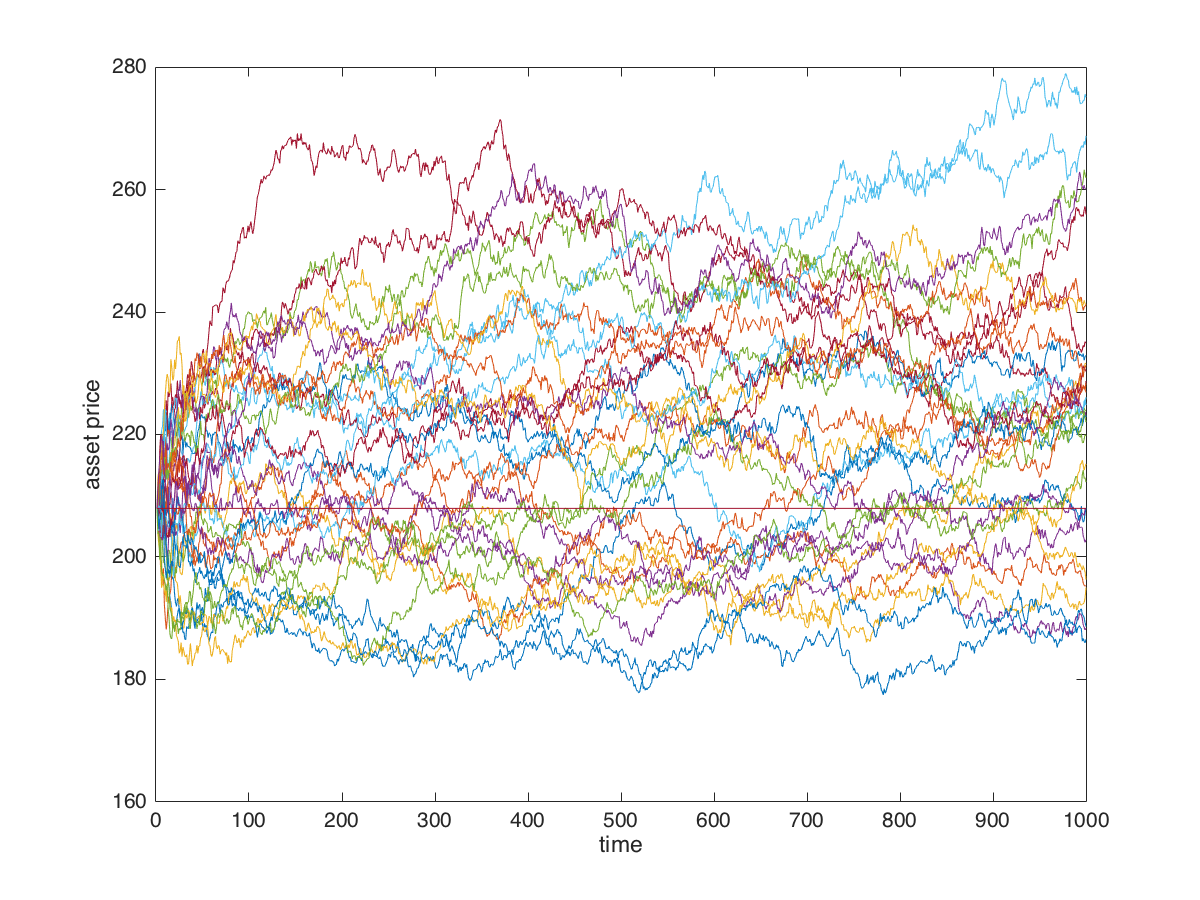
\includegraphics[width=0.80\textwidth]{../output/figures/chartHeston.png}
  \caption{Trajektorie procesu cen instrumentu bazowego}
  \label{fig:hestonAssetPaths}
\end{figure}

Na powyższym rysunku \ref{fig:hestonAssetPaths} widać wynik symulacji ceny opcji dla losowo wybranych przebiegów.
Z definicji symulacji Monte Carlo wynika, że poprawnym estymatorem ceny
opcji jest średnia ze wszystkich przebiegów.
Na rysunku zaznaczono również poziomą linią wartość punktu startowego, tzn. wartość 
aktywa bazowego w momencie zerowym. Wyraźnie widać, że średnia cena aktywa 
bazowego kształtuje się powyżej ceny wykupu opcji.

Tak jak w poprzednim podrozdziale, również w tym wyznaczono 
prawdziwą cenę opcji używając
modułu \textit{HestonExactLittleTrap}. Wyniki przedstawiono w tabeli
\ref{tab:littleTrapOption2}:

\begin{table}[ht!]
\centering 
\begin{tabular}{@{\hskip 0.5in}l |  @{\hskip 0.5in}r }
\toprule
$K$ & opcja nr 1 \\
\midrule
170.00 & 42.6957 \\
207.93 & 8.2123 \\
240.00 & 0.2102 \\
\bottomrule
\end{tabular}
\caption{Cena opcji na indeks S\&P500 otrzymana w wyniki implementacji 
         poprawki związanej z \textit{małą pułapką Hestona}}
\label{tab:littleTrapOption2}
\end{table}
Przyjmując takie same oznaczenia jak w podrozdziale 
\ref{sub:simulationNumericResult} wyniki symulacji dla opcji na indeks 
S\&P500 przedstawiają się w następujący sposób:
\begin{table}[ht!]
\centering
\resizebox{\textwidth}{!}{
\begin{tabular}{l l| >{\bfseries}rrr @{\hskip 0.5in} >{\bfseries}rrr @{\hskip 0.5in} >{\bfseries}r r r}
\toprule
{} & {} & EUL & Bias & SE & AND & Bias & SE & MAR & Bias & SE \\
\midrule
$\Delta$ & $N$ & {}  & {} & {} & K=170 \\
\midrule
10 & 1000 & 42.164 & -0.532 & 0.414 & 38.178 & -4.517 & 0.244 & 42.620 & -0.076 & 0.220 \\
20 & 4000 & 43.156 & 0.460 & 0.157 & 41.667 & -1.029 & 0.140 & 42.814 & 0.119 & 0.137 \\
40 & 16000 & 42.966 & 0.271 & 0.074 & 42.807 & 0.111 & 0.069 & 43.116 & 0.421 & 0.068 \\
80 & 64000 & 43.210 & 0.514 & 0.035 & 43.178 & 0.482 & 0.035 & 43.254 & 0.558 & 0.035 \\
160 & 256000 & 43.238 & 0.542 & 0.018 & 43.243 & 0.547 & 0.017 & 43.252 & 0.556 & 0.017 \\
320 & 1024000 & 43.250 & 0.554 & 0.009 & 43.271 & 0.575 & 0.009 & 43.268 & 0.572 & 0.009 \\
\midrule
{} & {} & {}  & {} & {} & K=207.93 \\
\midrule
10 & 1000 & 8.805 & 0.593 & 0.307 & 3.908 & -4.305 & 0.130 & 7.056 & -1.156 & 0.161 \\
20 & 4000 & 8.003 & -0.210 & 0.113 & 6.642 & -1.571 & 0.083 & 7.523 & -0.690 & 0.086 \\
40 & 16000 & 8.023 & -0.190 & 0.050 & 7.644 & -0.569 & 0.045 & 7.827 & -0.385 & 0.046 \\
80 & 64000 & 7.959 & -0.254 & 0.024 & 7.936 & -0.276 & 0.023 & 7.979 & -0.233 & 0.023 \\
160 & 256000 & 7.999 & -0.213 & 0.012 & 7.989 & -0.223 & 0.012 & 7.989 & -0.223 & 0.012 \\
320 & 1024000 & 8.005 & -0.207 & 0.006 & 8.010 & -0.202 & 0.006 & 8.015 & -0.198 & 0.006 \\
\midrule
{} & {} & {} & {} & {} & K=240 \\
\midrule
10 & 1000 & 0.175 & -0.036 & 0.045 & 0.000 & -0.210 & 0.000 & 0.000 & -0.210 & 0.000 \\
20 & 4000 & 0.017 & -0.193 & 0.006 & 0.000 & -0.210 & 0.000 & 0.000 & -0.210 & 0.000 \\
40 & 16000 & 0.000 & -0.210 & 0.000 & 0.000 & -0.210 & 0.000 & 0.000 & -0.210 & 0.000 \\
80 & 64000 & 0.000 & -0.210 & 0.000 & 0.000 & -0.210 & 0.000 & 0.000 & -0.210 & 0.000 \\
160 & 256000 & 0.000 & -0.210 & 0.000 & 0.000 & -0.210 & 0.000 & 0.000 & -0.210 & 0.000 \\
320 & 1024000 & 0.000 & -0.210 & 0.000 & 0.000 & -0.210 & 0.000 & 0.000 & -0.210 & 0.000 \\
\bottomrule
\end{tabular}
}
\caption{Porównanie schematów dyskretyzacji na przykładzie opcji na indeks S\&P500}
\label{tab:optionDiscretizationSP}
\end{table}

Jak wynika z powyższej tabeli, dla wszystkich trzech metod dyskretyzacji 
otrzymujemy podobne wyniki. Jedynie dla niskiej wartości $\Delta$ oraz $N$ rysuje się 
przewaga dyskretyzacji Eulera: wyznaczona tym sposobem wartość opcji jest dużo
dokładniejsza niż dla dyskretyzacji metodami Andersena.



\subsection{Płaszczyzna zmienności implikowanej}

W podrozdziale \ref{sub:simulationNumericResult} wyznaczono płaszczyznę
zmienności implikowanej dla zadanego zbioru cen wykupu oraz terminów do wygaśnięcia. 
Podobną procedurę przeprowadzono dla opcji na indeks
S\&P500. W rezultacie otrzymano:

\begin{figure}[ht!]
  \centering
  \includegraphics[width=0.80\textwidth]{../src/HestonMATLAB/impliedvol/figs/hestonVolSurfaceExampleSAndP.pdf}
  \caption{Płaszczyzna zmienności implikowanej dla indeksu $S\&P$500}
  \label{fig:volatilitySurface}
\end{figure}
Dla opcji o bliskim terminie do wygaśnięcia ponownie widzimy silny \textit{grymas} 
zmienności. Dla opcji o dalekim terminie wykupu, np. $T=3$ jest on 
bardzo nieznaczny.

\subsection{Współczynniki greckie}

Na koniec podrozdziału przedstawimy zachowanie się modelu Hestona dla jednego, wybranego współczynnika 
greckiego, a mianowicie dla $\Theta$.

\textit{Theta}, jako współczynnik cen opcji w zależności od upływającego czasu:
\begin{equation}
  \Theta = - \frac{\delta V}{\delta T}
\end{equation}
Rysunek \ref{fig:hestonTimeToExpiry} przedstawia zachowanie się cen opcji wraz z rosnącym czasem do 
wygaśnięcia opcji. Dla pierwszego wykresu czas do wygaśnięcia wynosi pół roku, natomiast dla 
ostatniego wynosi 6 lat. 

\begin{figure}[ht!]
  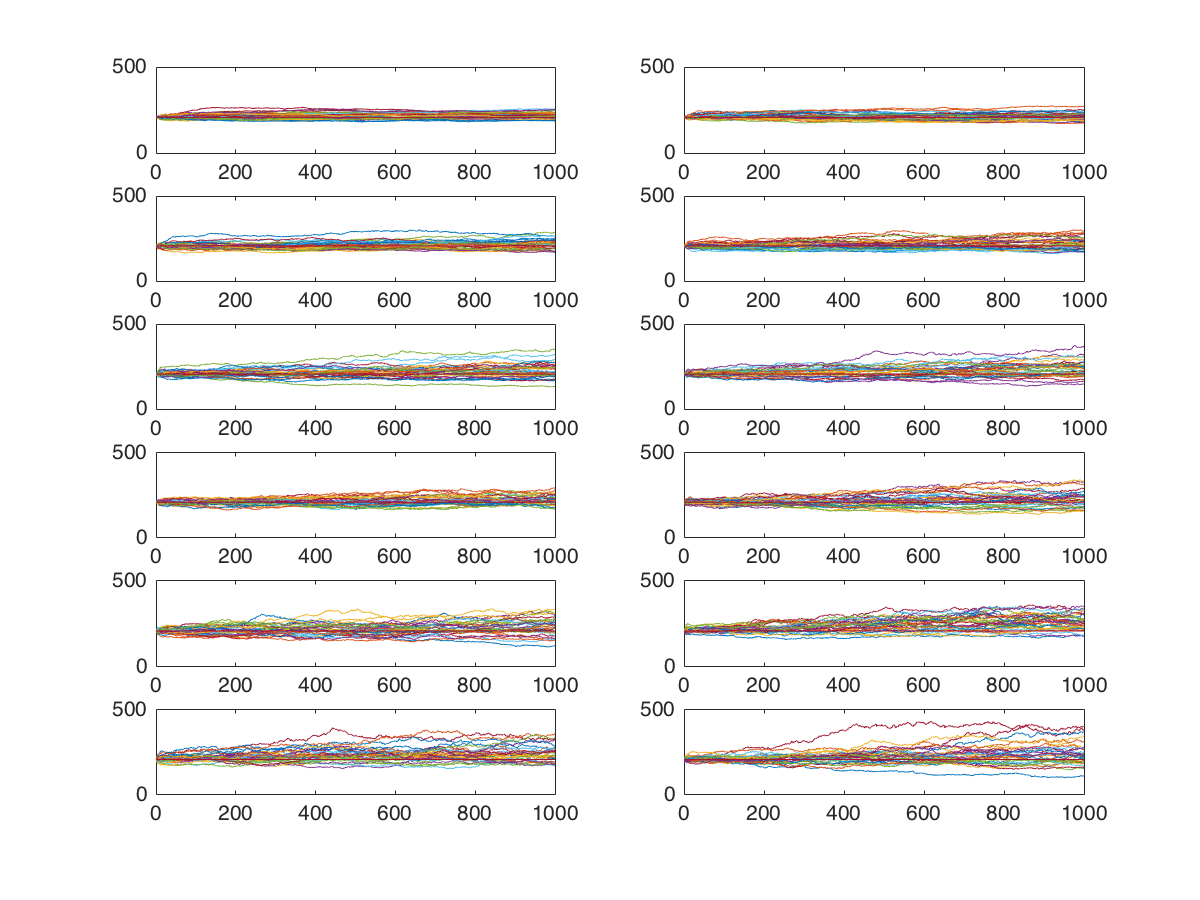
\includegraphics[width=1.00\textwidth]{../output/figures/hestonTimeToExpiry.pdf}
  \caption{Cena instrumentu bazowego w modelu Hestona w zależności od czasu do wygaśnięcia opcji}
  \label{fig:hestonTimeToExpiry}
\end{figure}


Jak można zauważyć, wraz ze spadającym czasem do wygaśnięcia maleje potencjalny rozrzut cen aktywa 
bazowego w momencie wygaśnięcia opcji.
Jest to zgodne z intuicją. Opcje, których cena jest zależna od zmienności instrumentu bazowego, 
w krótszym okresie czasu będą mniej warte od tych z dłuższym okresem do wygaśnięcia.






%===========================================================================
%                             Zakończenie
%===========================================================================
\cleardoublepage
\phantomsection
\chapter*{Podsumowanie}\label{r:ending}
\addcontentsline{toc}{chapter}{Podsumowanie} \markboth{Finish}{}

Celem niniejszej pracy było porównanie modeli służących do wyceny
opcji oraz implementacja modelu Hestona, który wylicza wartość opcji biorąc
pod uwagę brak stałości w czasie zmienności, jednego z podstawowych parametrów
mającego wpływ na wycenę opcji. 

Pierwszym modelem służącym do wyceny opcji jest model Blacka-Scholesa, który jest
najprostszym modelem do wyceny opcji i porównano go do efektywności modelu 
Hestona. 

Model Hestona, który jest bardziej zaawansowany koncepcyjnie, jest jednocześnie 
bardziej skomplikowany obliczeniowo. Wynika to z faktu, że ma on kilka dodatkowych
parametrów, które należy wyznaczyć na podstawie informacji z rynku. Proces wyznaczania tych 
parametrów, nazwany procesem kalibracji, jest o wiele bardziej skomplikowany w przypadku 
modelu Hestona, ponieważ tutaj jest to zadanie optymalizacyjne, natomiast w przypadku modelu
Blacka-Scholesa jest to zadanie algebraiczne.

Szczegółowo opisano również, w jaki sposób należy zastosować symulację Monte Carlo do 
wygenerowania ceny opcji zgodnej z modelem Hestona. Krytycznym punktem okazał się być
proces dyskretyzacji procesu losowego. Przedstawiono trzy schematy: pierwszy - naiwny, nazwany
dyskretyzacją Eulera, drugi - bardziej dokładny, którego wynikiem było powstanie 
algorytmu Andersena oraz trzeci, który jest ulepszeniem wspomnianego algorytmu 
Andersena

Z badań empirycznych jasno wynika, że założenie o stałości zmienności w czasie nie jest 
prawdziwe dla danych rzeczywistych. Ponadto, przeprowadzono wycenę opcji 
dla modelu Hestona stosując różne schematy dyskretyzacji.
Wszystkie trzy metody dyskretyzacji się 
sprawdzają, jednak największą dokładność osiąga schemat Andersena wraz
z poprawką martyngałową.


Podsumowując, można stwierdzić, że model Hestona jest o wiele bardziej zaawansowanym
narzędziem do wyceny opcji niż model Blacka-Scholesa. Uwzględniając zróżnicowanie zmienności 
w czasie sprawia, że cena opcji jest bardziej dokładna. Cena jaką za to płacimy,
jest o wiele większe skomplikowanie modelu, zarówno w sferze koncepcyjnej, jak i 
implementacyjnej. Ze względu na konieczność wieloparametrowej kalibracji modelu, 
model ten jest o wiele bardziej czasochłonny obliczeniowo, w porównaniu do np. modelu Blacka-Scholesa.

%===========================================================================
%                             Appendix - kody zrodlowe
%===========================================================================
\cleardoublepage
\phantomsection
\appendix

\chapter{Opis kodu źródłowego}

W tym rozdziale zostanie przedstawiona implementacja wybranych zagadnień przedstawionych w 
pracy magisterskiej. Kod źródłowy został napisany w dwóch językach programowania: 
\begin{enumerate}
  \item \textit{C++}
  \item \textit{Matlab}
\end{enumerate}
W tym pierwszym zaimplementowano następujące moduły:
\begin{itemize}
  \item model Hestona i różne sposoby jego dyskretyzacji
  \item model Blacka-Scholesa
  \item generator liczb z rozkładu normalnego
  \item symulację Monte Carlo dla modelu Hestona
\end{itemize}
Z kolei w języku \textit{Matlab} zaimplementowano kalibrację modelu Hestona do cen opcji pochodzących
z danych giełdowych.

Wszystkie zaimplementowane moduły zostały wykonane na maszynie o następujących parametrach:
\begin{enumerate}
  \item procesorze \textit{Intel Core i5, 2.6 GHz}
  \item pamięci \textit{8GB}
  \item systemie operacyjnym \textit{OS X El Capitan 10.11.3}
\end{enumerate}


\section{Model Hestona}
Na schemacie \ref{fig:currencyRisk} widać poszczególne klasy zaimplementowane w 
ramach modułu wyliczającego cenę opcji zgodną z modelem Hestona.
Klasą bazową, po której wszystkie inne dziedziczą, jest klasa \textit{Heston}.
Jest ona bezpośrednią nadklasą dla innych klas definiujących 
odmienne podejścia do wyceny opcji zgodnej z modelem Hestona:
\begin{enumerate}
  \item symulacji Monte Carlo (klasa \textit{HestonMC})
  \item wzoru w postaci jawnej (klasa \textit{HestonExact})
\end{enumerate}

Klasa \textit{HestonExact} zawiera w sobie implementację wzoru formie jawnej na cenę opcji.
Dziedziczy po niej klasa \textit{HestonExactLittleTrap}, która definiuje 
poprawkę związaną z \textit{małą pułapką Hestona}. Dzięki tej klasie 
otrzymujemy implementację jawnego wzoru na cenę opcji, która jest w o wiele
mniejszym stopniu podatna na błędy numeryczne.

Z kolei klasa \textit{HestonMC} definiuje jedynie interfejs jaki muszą spełniać klasy po niej 
dziedziczące.
Abstrakcyjna \textit{HestonMC} jest z kolei klasą bazową dla następujących klas:
\begin{enumerate}
  \item \textit{HestonAndersen} 
  \item \textit{HestonEuler} 
\end{enumerate}
Na schemacie \ref{fig:currencyRisk} widać również dodatkową klasę
\textit{HestonAndersenMartingale}. Jest to klasa implementująca 
poprawkę martyngałową dla modelu Hestona, którą przedstawiono 
w rozdziale \ref{chap:monteCarlo}.


\begin{figure}
  \centering  
  \includegraphics[width=1.00\textwidth]{../output/diagramms/HestonDiagramm.pdf}
  \caption{Drzewo dziedziczenia dla modułu wyliczającego 
  cenę opcji wg różnych metodologii dla modelu Hestona.}\label{fig:currencyRisk}
\end{figure}

Klasa (\textit{HestonMC})
jest klasą bazową dla klas wykonujących symulację Monte Carlo zgodnie z 
przyjętym schematem dyskretyzacji. Definiuje ona dwie dodatkowe metody: \textit{simulateVolPath} oraz 
\textit{simulateSpotPath}.

\section{Interfejs abstrakcyjnych klas \textit{Heston} oraz \textit{HestonMC}}
W projekcie zostały zaimplementowane dwie abstrakcyjne klasy \textit{Heston} oraz \textit{HestonMC}.
Pierwsza z nich stanowi klasę bazową dla całej struktury drzewa dziedziczenia. 
\begin{listing}[H]
\inputminted[mathescape, linenos, numbersep=5pt, bgcolor=bg, frame=lines, framesep=2mm]{cpp}
{../src/HestonCPP/src/main/cpp/heston/header/Heston.h}
\caption{Plik nagłówkowy dla klasy \textit{Heston}}
\end{listing} 
\begin{listing}[H]
\inputminted[mathescape, linenos, numbersep=5pt, bgcolor=bg, frame=lines, framesep=2mm]{cpp}
{../src/HestonCPP/src/main/cpp/heston/header/HestonMC.h}
\caption{Plik nagłówkowy dla klasy definiującej interfejs symulacji Monte Carlo}
\end{listing} 




\clearpage
\subsection{Schemat Eulera}

W tym podrozdziale zostanie przedstawiony kod do wyceny opcji zgodnie z dyskretyzacją Eulera.
Na rysunku przedstawiono plik źródłowy klasy\textit{HestonEuler}. Jest ona rozszerzeniem klasy 
HestonMC, a więc udostępnia ona interfejs swoich nadklas. 



\begin{listing}[H]
\inputminted[mathescape, linenos, numbersep=5pt, bgcolor=bg, frame=lines, framesep=2mm]{cpp}
{../src/HestonCPP/src/main/cpp/heston/header/HestonEuler.h}
\caption{Plik nagłówkowy klasy \textit{HestonEuler}.}
\end{listing} 
Kod źródłowy \label{lst:Eulercpp} przedstawia z kolei implementację dwóch metod:
\begin{enumerate}
  \item \textit{HestonEuler::simulateVolPath}
  \item \textit{HestonEuler::simulateSpotPath}
\end{enumerate}

\begin{listing}[H]
\inputminted[mathescape, linenos, numbersep=5pt, bgcolor=bg, frame=lines, framesep=2mm]{cpp}
{../src/HestonCPP/src/main/cpp/heston/src/HestonEuler.cpp}
\caption{Implementacja metod dla schematu Eulera.}
\label{lst:Eulercpp} 
\end{listing}




\clearpage
\subsection{Schemat Andersena}
W tym punkcie podana zostanie implementacja kolejnego schematu dyskretyzacji, schematu 
Andersena. Zostały podane dwa
pliki: jeden to plik nagłówkowy, a drugie z implementacją odpowiednich metod.
Klasa \textit{HestonAndersen} zawiera jedną dodatkową 
metodę:
\begin{itemize}
   \item \textit{HestonAndersen::modifiedExpInvCDF}
 \end{itemize} 
Jest to funkcja, która wylicza wartość odwrotnej dystrybuanty dla zmodyfikowanego rozkładu 
wykładniczego.
\begin{listing}[H]
\inputminted[mathescape, linenos, numbersep=5pt, bgcolor=bg, frame=lines, framesep=2mm]{cpp}
{../output/listings/HestonAndersen.h}
\caption{Schemat generowania trajektorii procesu aktywa bazowego wraz z poprawką
martyngałową}
\end{listing}
\begin{listing}[H]
\inputminted[mathescape, linenos, numbersep=5pt, bgcolor=bg, frame=lines, framesep=2mm]{cpp}
{../output/listings/HestonAndersen.cpp}
\caption{Metoda \textit{simulateVolPath} z jednoczesnym wyznaczeniem poprawki martyngałowej}
\end{listing}  
Podobnie jak dla dyskretyzacji Eulera definiujemy metody 
\begin{enumerate}
  \item \textit{HestonEuler::simulateVolPath},
  \item \textit{HestonEuler::simulateSpotPath}.
\end{enumerate}

Metoda \textit{HestonEuler::simulateVolPath} oblicza trajektorię procesu zmienności, 
natomiast metoda \textit{HestonEuler::simulateSpotPath} wyznacza trajektorię procesu aktywa
bazowego.
\begin{listing}[H]
\inputminted[mathescape, linenos, numbersep=5pt, bgcolor=bg, frame=lines, framesep=2mm]{cpp}
{../output/listings/HestonAndersen2.cpp}
\caption{Metoda \textit{simulateSpotPath} wyznaczająca trajektorię aktywa bazowego.}
\end{listing}   
Dla porządku podana została również definicja metody zwracającej wartość odwrotnej 
dystrybuanty dla zmodyfikowanego rozkładu wykładniczego. Metoda jest widoczna na kodzie źródłowym 
\ref{lst:ModifiedExpInvCDF}.

\begin{listing}[H]
\inputminted[mathescape, linenos, numbersep=5pt, bgcolor=bg, frame=lines, framesep=2mm]{cpp}
{../output/listings/ModifiedExpInvCDF.cpp}
\caption{Funkcja wyliczająca wartość odwrotnej dystrybuanty dla zmodyfikowanego rozkładu 
wykładniczego}
\label{lst:ModifiedExpInvCDF} 
\end{listing}





\clearpage
\subsection{Schemat Andersena z poprawką Martyngałową}
W poprzednim punkcie zaimplementowano schemat Andersena. 
Niestety, proces aktywa bazowego w tym schemacie nie jest martyngałem.
Algorytm ten można jednak usprawnić tak, aby własność martyngału była spełniona.
Definiuję się zmienną $k_0^*$, która zastępuje zmienną $k_0$: 
\begin{listing}[H]
\inputminted[mathescape, linenos, numbersep=5pt, bgcolor=bg, frame=lines, framesep=2mm]{cpp}
{../output/listings/HestonAndersenMartingaleSpot.cpp}
\caption{Schemat generowania trajektorii procesu aktywa bazowego wraz z poprawką
martyngałową}
\end{listing}  

Klasa \textit{HestonAndersenMartingale} jest podklasą klasy \textit{HestonAndersen}, 
dlatego nie musimy implementować niektórych metod, jak np. metodę wyliczającą trajektorię procesu
wariancji. 
Klasa \textit{HestonAndersenMartingale} udostępnia ponadto metodę do wyliczenia parametru $k_0^*$.
Nosi ona nazwę \textit{calcMartingaleCorr}. 
Poniżej podajemy implementację tej metody, która wylicza poprawkę martyngałową 
dla każdego punktu realizacji procesu aktywa bazowego.

\begin{listing}[H]
\inputminted[mathescape, linenos, numbersep=5pt, bgcolor=bg, frame=lines, framesep=2mm]{cpp}
{../output/listings/HestonAndersenMartingaleMart.cpp}
\caption{Metoda wyliczająca poprawkę martyngałową}
\end{listing}



\clearpage
\subsection{Wycena opcji przy pomocy wzoru w formie jawnej}
W tym rozdziale zostaną przedstawione kody źródłowe dla alternatywnego podejścia 
wyceny opcji w modelu Hestona. Zamiast polegać na niedeterministycznej metodzie
Monte Carlo, zostanie użyty wzór w formie jawnej. Plik nagłówkowy dla tej klasy
został przedstawiony poniżej.
\begin{listing}[H]
\inputminted[mathescape, linenos, numbersep=5pt, bgcolor=bg, frame=lines, framesep=2mm]{cpp}
{../output/listings/HestonExact.h}
\caption{Plik nagłówkowy dla klasy \textit{HestonExact}}
\end{listing}  
\begin{listing}[H]
\inputminted[mathescape, linenos, numbersep=5pt, bgcolor=bg, frame=lines, framesep=2mm]{cpp}
{../output/listings/HestonExact1.cpp}
\caption{Implementacja metod klasy \textit{HestonExact}, część 1.}
\end{listing}  
\begin{listing}[H]
\inputminted[mathescape, linenos, numbersep=5pt, bgcolor=bg, frame=lines, framesep=2mm]{cpp}
{../output/listings/HestonExact2.cpp}
\caption{Implementacja metod klasy \textit{HestonExact}, część 2.}
\end{listing}




\clearpage
\subsection{Implementacja modułu \textit{HestonExactLittleTrap}}
Sekcja ta przedstawia kod źródłowy dla opisanej w rozdziale, implementacji wzoru w formie jawnej
na wycenę opcji. 
\begin{listing}[H]
\inputminted[mathescape, linenos, numbersep=5pt, bgcolor=bg, frame=lines, framesep=2mm]{cpp}
{../output/listings/HestonExactLittleTrap.h}
\caption{Plik nagłówkowy dla klasy \textit{HestonExactLittleTrap}.}
\end{listing}  
\begin{listing}[H]
\inputminted[mathescape, linenos, numbersep=5pt, bgcolor=bg, frame=lines, framesep=2mm]{cpp}
{../output/listings/HestonExactLittleTrap.cpp}
\caption{Implementacja metod dla klasy \textit{HestonExactLittleTrap}.}
\end{listing}  



%===========================================================================
%                             Polar generator
%===========================================================================
\clearpage
\section{Generator liczb z rozkładu normalnego}
Przedstawiony poniżej kod źródłowy przedstawia plik nagłówkowy definiujący interfejs 
generatora liczb losowych z rozkładu normalnego. 
\begin{listing}[H]
\inputminted[mathescape, linenos, numbersep=5pt, bgcolor=bg, frame=lines, framesep=2mm]{cpp}
{../src/HestonCPP/src/main/cpp/random/PolarGenerator.h}
\caption{Plik nagłówkowy klasy \textit{PolarGenerator}.}
\end{listing} 
Klasa ta została utworzona zgodnie z kreacyjnym wzorcem projektowym \textit{singleton}. 
Główną zaletą tego wzorca jest to, że pozwalamy na utworzenie tylko jednego obiektu danej 
klasy, co jest istotne w przypadku implementacji konstruktora klasy definiującej
generator liczb pseudolosowych.
Implementacja wzorca została wykonana zgodnie ze schematem podanym przez Meyersa \cite{Meyers}, 
która jest bezpieczna w środowisku wielowątkowym (\textit{ang. thread-safe}).
\begin{listing}[H]
\inputminted[mathescape, linenos, numbersep=5pt, bgcolor=bg, frame=lines, framesep=2mm]{cpp}
{../src/HestonCPP/src/main/cpp/random/PolarGenerator.cpp}
\caption{Implementacja interfejsu klasy \textit{PolarGenerator}.}
\label{lst:PolarGeneratorcpp}
\end{listing} 
Kod źródłowy nr \ref{lst:PolarGeneratorcpp} przedstawia implementację konstruktora oraz metody
generującej liczby z rozkładu normalnego \textit{genNorm()} \cite{joshi2008c++}.


%===========================================================================
%                             Model Blacka-Scholesa
%===========================================================================
\clearpage
\section{Model Blacka-Scholesa}
Kod źródłowy nr \ref{lst:BlackScholesh} przedstawia plik nagłówkowy dla implementacji 
modelu Blacka-Scholesa. Implementacja ta jest użyta do porównania wartości opcji dla 
modelu Blacka-Scholesa i modelu Hestona.
\begin{listing}[H]
\inputminted[mathescape, linenos, numbersep=5pt, bgcolor=bg, frame=lines, framesep=2mm]{cpp}
{../src/HestonCPP/src/main/cpp/bs/MCBlackScholes.h}
\caption{Interfejs klasy wyliczającej wartość opcji wg modelu Blacka-Scholesa.}
\label{lst:BlackScholesh}
\end{listing} 
Kod źródłowy \ref{lst:BlackScholescpp} przedstawia konstruktor klasy \textit{MCBlackScholes} 
oraz implementację metody \textit{simulate} (na podstawie \cite{joshi2008c++}).
\begin{listing}[H]
\inputminted[mathescape, linenos, numbersep=5pt, bgcolor=bg, frame=lines, framesep=2mm]{cpp}
{../src/HestonCPP/src/main/cpp/bs/MCBlackScholes.cpp}
\caption{Implementacja klasy \textit{MCBlackScholes}.}
\label{lst:BlackScholescpp}
\end{listing} 


%===========================================================================
%                         Symulacja Monte Carlo
%===========================================================================
\clearpage
\section{Symulacje Monte Carlo}
Kod źródłowy \ref{lst:MonteCarloh} przedstawia plik nagłówkowy dla implementacji symulacji 
Monte Carlo dla modelu Hestona. Plik definiuje interfejs jaki musi spełniać
implementacja symulacji Monte Carlo. Najważniejszą publiczną metodą jest metoda \textit{simulate}, 
dla której jako parametr przekazujemy odpowiedni schemat dyskretyzacji modelu Hestona 
oraz opcję do wyceny. 
Ponadto zdefiniowany jest konstruktor klasy, który jako parametry przyjmuje dwie zmienne:
\textit{simulationTrials} oraz \textit{timeSteps}.
Pierwsza ze zmiennych definiuje ile razy wykonujemy pojedynczą symulację, natomiast druga 
definiuje liczbę kroków w pojedynczej symulacji. Innymi słowy, czas wygaśnięcia opcji 
podzielony przez liczbę kroków definiuje nam jednostkowy przyrost czasu.
\begin{listing}[H]
\inputminted[mathescape, linenos, numbersep=5pt, bgcolor=bg, frame=lines, framesep=2mm]{cpp}
{../src/HestonCPP/src/main/cpp/mc/MonteCarloSimulation.h}
\caption{Plik nagłówkowy dla symulacji Monte Carlo}
\label{lst:MonteCarloh}
\end{listing} 
Kod źródłowy nr \ref{lst:MonteCarlocpp} przedstawia główną funkcję użytą w tym celu. 
Zastosowano w niej prostą metodę Monte Carlo wraz ze schematem dyskretyzacji Eulera. 
Parametrami dla funkcji \textit{simulateHeston} są dwa wektory, pierwszy zawierający
parametry modelu Hestona, natomiast drugi parametry opcji, której cenę chcemy wyznaczyć. 
Główną częścią pokazanego algorytmu jest pętla w liniach 20-24, która stanowi faktyczną symulację
Monte-Carlo. Najpierw generujemy w niej skorelowane ciągi losowe mające rozkład normalny, 
a następnie na ich podstawie generujemy kolejno trajektorię zmienności oraz trajektorię aktywa
bazowego. W linii 24 bierzemy wartość aktywa bazowego w momencie $T$ i na tej podstawie obliczamy dla
tej wartości kwotę wypłaty opcji. Aby otrzymać wartość opcji, musimy wziąć średnią z wypłat i
zdyskontować ją na moment zerowy, co jest widoczne w liniach 27-28.

\begin{listing}[H]
\label{lst:MCHeston} 
\inputminted[mathescape, linenos, numbersep=5pt, bgcolor=bg, frame=lines, framesep=2mm]{cpp}
{../output/listings/MonteCarloSimulation.cpp}
\caption{Symulacja Monte Carlo dla modelu Hestona  \cite{HallsMoore}}
\label{lst:MonteCarlocpp}
\end{listing}  

%===========================================================================
%                         Kalibracja do danych rynkowych
%===========================================================================
\clearpage
\section{Kalibracja do danych rynkowych}
Kod źródłowy \ref{lst:MonteCarloh} przedstawia główny program wykonujący
kalibrację do danych rynkowych.

\begin{listing}[H]
\inputminted[mathescape, linenos, numbersep=5pt, bgcolor=bg, frame=lines, framesep=2mm]{matlab}
{../output/listings/calibration.m}
\caption{Skrypt kalibrujący model Hestona do danych rynkowych}
\label{lst:MonteCarloh}
\end{listing}



%===========================================================================
%                             Listingi
%===========================================================================
\cleardoublepage
\phantomsection
\addcontentsline{toc}{chapter}{Spis rysunków}{\listoffigures}
\cleardoublepage
\phantomsection
\addcontentsline{toc}{chapter}{Spis tabel}{\listoftables}
\cleardoublepage
\phantomsection
\addcontentsline{toc}{chapter}{Spis kodów źródłowych}{\listoflistings}
\cleardoublepage
\phantomsection
\addcontentsline{toc}{chapter}{Spis algorytmów}{\listofalgorithms}
\cleardoublepage
\phantomsection
\addcontentsline{toc}{chapter}{Bibliografia}{\printbibliography}

\end{document} 